%%=======================================================================
%% The Axis of the Sign Is Not Scale
%% 由 mm_sys/make_main.py + build_en.py 自动生成，请勿手工编辑。
%%=======================================================================
%% 本刊用编号制参考文献（方括号）；sn-basic + Numbered 即产出该制式。
\documentclass[pdflatex,sn-basic,Numbered]{sn-jnl}

\usepackage{graphicx}
\usepackage{multirow}
\usepackage{amsmath,amssymb,amsfonts}
\usepackage{amsthm}
\usepackage{mathrsfs}
\usepackage{xcolor}
\usepackage{textcomp}
\usepackage{booktabs}
\usepackage{tabularx}
\usepackage{listings}

\theoremstyle{thmstyleone}
\newtheorem{theorem}{Theorem}
\newtheorem{proposition}[theorem]{Proposition}
\theoremstyle{thmstyletwo}
\newtheorem{example}{Example}
\newtheorem{remark}{Remark}
\theoremstyle{thmstylethree}
\newtheorem{definition}{Definition}

%% sn-jnl 的 \orcid 展开成 \includegraphics{Orcidlogo.eps}，该文件不在本目录，
%% 编译会因缺图失败。这里重定义成文本形式的标准 iD 标记。
\renewcommand{\orcid}[1]{\href{#1}{\,\textsuperscript{iD}}}

%% 本文排版自定义宏（与中文版同名，保证两版公式一致）
\newcommand{\Dstar}{\mathcal{D}^{*}}
\newcommand{\PKD}{\mathrm{PKD}}
\newcommand{\dlt}{\Delta}
\newcommand{\pp}{\,\mathrm{pp}}
\DeclareRobustCommand{\code}[1]{\texttt{\spaceskip=0pt plus 0.4em\relax#1}}
\DeclareRobustCommand{\codesplit}[1]{\texttt{\spaceskip=0pt plus 0.4em\relax#1}}
\newcommand{\pthbreak}[1][0pt]{\hspace{0pt}\allowbreak\hspace{0pt}}

%% 本文有几张较高的组合图，默认 \topfraction=0.7 会让它们排不进页顶，
%% 一路被推到文末。这里放宽页顶容图比例。
\renewcommand{\topfraction}{0.85}
\renewcommand{\bottomfraction}{0.7}
\renewcommand{\textfraction}{0.07}
\renewcommand{\floatpagefraction}{0.75}

\raggedbottom

\begin{document}

\title[The axis of the sign is not scale]{%
The Axis of the Sign Is Not Scale: Evaluation Protocol Determines the
Sign of the Scale Effect in Multimodal RAG}

\author[1]{\fnm{Lin} \sur{Chen}}\email{chenlin@sdu.edu.cn}

\author*[1]{\fnm{Zhen} \sur{Li}\orcid{https://orcid.org/0009-0008-4719-9631}}\email{jens@sdu.edu.cn}

\author[1]{\fnm{Bin} \sur{Wang}}\email{wangbin@sdu.edu.cn}

\author[2]{\fnm{Jie} \sur{Liu}}\email{liuj1687@chinaunicom.cn}

\affil*[1]{\orgdiv{Digital Intelligence Support Research Institute},
\orgname{Shandong University},
\orgaddress{\street{No. 27 Shanda South Road}, \city{Jinan},
\postcode{250100}, \state{Shandong}, \country{China}}}

\affil[2]{\orgname{China Unicom (Tianjin) Industrial Internet Co., Ltd.},
\orgaddress{\city{Tianjin}, \postcode{300110}, \country{China}}}

\abstract{When retrieved evidence conflicts with a model's parametric knowledge, behaviour is no longer governed by task difficulty alone. Holding the conflict construction, the adjudication criterion, the models and the samples fixed, we vary exactly one variable: the strength with which the system prompt authorises parametric knowledge, pre-registered as seven ordered stances from weak to strong. On 927 controlled counterfactually edited conflict samples, an anchoring protocol guarantees that every scale point genuinely knows the fact at issue ($|D^*| = 649$). The result is that the sign of the scale effect is determined by the evaluation protocol, not by scale. The $\Delta$ of the seven stances crosses zero, with signs running from negative to positive along the pre-registered authorisation order, spanning 47.5 to 56.5 percentage points, and replicating independently on two model families. The sign flip is decided by the mid-ladder stance \code{ctx\_hedge}, so the ordering is not a monotone gradient, and the structure holds only under free generation. Methodologically we report three directional measurement biases—explicit rejection misread as undecidable, denominator collapse misread as the strongest effect, and position preference masquerading as content judgment—each of which is sufficient to let the same data support the opposite conclusion.}

\keywords{knowledge conflict, multimodal RAG, evaluation protocol,
scale effect, sign crossing, measurement bias}

\maketitle

% 由 build_en.py 自动生成，请勿手工编辑。

\section{Introduction}\label{sec:1}

Retrieval-augmented generation delegates facts the parameters cannot hold to external evidence. Once retrieved content conflicts with parametric knowledge, behaviour is no longer determined by task difficulty: for the same question and model, the answer may follow retrieved content or the parameter, and which one is chosen depends on how the prompt is written. This is not a corner case—retrieved evidence may itself be wrong, and whether the model holds to parametric knowledge decides whether the system keeps that error out or accepts it wholesale. Multimodal settings push the problem further: image evidence, retrieved text, and parametric facts may conflict pairwise.

A recent body of work measures this choice: ConflictBank constructs samples in which context and parametric knowledge conflict \cite{ref1}, ClashEval reports adoption of incorrect retrieved content above 60\% \cite{ref2}, and the multimodal sycophancy benchmark PENDULUM extends the measurement to vision-language models \cite{ref3}. These establish that models are swayed by conflicting context and leave the next question: does this swaying improve or worsen as capability increases?

The natural guess is that it improves—parametric knowledge grows with scale, so models should better identify incorrect evidence. But testing this carries an easily overlooked precondition: scale must be the only variable that changes. In practice the prompt changes too, some saying "answer only from the context", others "if the context is unreliable, rely on your own knowledge". If the degree to which the template authorises parametric knowledge itself changes behaviour, attributing a difference between scales to scale may amount to measuring the template.

This paper turns the question into a decidable experiment: fixing the conflict construction, the decision criterion, the models, and the samples, and varying a single variable—the strength with which the system prompt authorises parametric knowledge, pre-registered by semantics from weak to strong into seven levels, from "use only the context" to "rely on your own knowledge". On 927 conflict samples from controlled counterfactual edits we measure the proportion of cases where the model follows parametric knowledge at each scale and stance. An anchoring protocol ensures every scale under test in fact knows the fact—if a small model does not know it, its "not following parametric knowledge" under conflict is not a product of choice. This shrinks 927 samples to 649 and isolates the capability gap from the trivial explanation that larger models simply know a few more facts.

The result is that the sign of the scale effect is determined not by scale but by stance. Across two model families, weakly authorising stances make larger models more inclined to follow the context (\code{ctx\_only} at $-27.3$ and $-8.4$ pp), while strongly authorising stances make them likelier to hold to parametric knowledge (\code{prior} at $+28.0$ and $+33.7$ pp). The $\Delta$ of both families crosses zero, the sign is ordered from negative to positive along the pre-registered authorisation order, and decomposition into adjacent scale pairs shows early saturation rather than smooth growth.

That the signs are ordered is not a monotonic gradient, and this is the paper's most critical and most easily misread point. What decides the flip is not the rule "the stronger the authorisation, the more positive the effect": the mid-sequence stance \code{ctx\_hedge} explicitly commands "when the context is unreliable, rely on your own knowledge" and yields $+29.2$ pp for the Qwen3 family, whereas the semantically weaker \code{neutral} stance that follows yields only $+1.5$ pp. Which stance the sign lands on is decided jointly by that stance's output form and the decision criterion—the "protocol" rather than the "stance semantics" of the title. This cell is also the least trustworthy in magnitude, yet removing it entirely leaves the sign sequence of both families unchanged (first two negative, last four positive), the span falls only from 56.5 to 55.3 pp, and the Qwen3 rank correlation rises from 0.643 to 1.000. The least trustworthy cell is not load-bearing.

The conclusion carries a necessary qualification that is itself part of the result: it holds only under the free-generation format. Under the forced-choice template of two published works, the scale effects of all four conditions stay within $-4$ pp, uniformly negative, and do not change with the framing (\ref{sec:4-5}).

At the methodological level we report three measurement problems not previously addressed systematically, each of which would lead the same data to conclusions of opposite direction. First, the criterion misrecords explicit rejection as undecidable: when a model outputs "the context is incorrect, the origin of X is Y" it names both values and is judged undecidable and excluded, yet such answers are the most unambiguous cases of following parametric knowledge; exclusions rise with scale, and after correction the \code{PKD} of one stance rises from 0.359 to 0.960. Second, denominator collapse is misread as the strongest effect: paired decidable samples for the same stance collapse from 584 to 1 across three criteria, and when the denominator reaches single digits $\Delta$ can only take degenerate values, yet in the table it looks like the strongest cell; we therefore stipulate that cells with $n<50$ are not counted in the span and sign comparisons. Third, position preference can completely override content: under the forced-choice format, rerunning after swapping the option contents yields a position preference of $+0.961$, so the high accuracy is a product of position rather than content judgement. None of the three disappears when the criterion or template is changed, and each has at some point reversed the direction of one of our own conclusions.

The contributions are three. First, the measurement conclusion that the sign of the scale effect is a function of the evaluation protocol, turned into a decidable design: seven pre-registered stances × five scale points × two model families, with $\Delta$ crossing zero and the signs ordered, independently reproduced across the two families. Second, the three-way conflict construction of controlled counterfactual edits plus an anchoring protocol, separating "whether the model resists tampered retrieved evidence" from "whether the model knows the fact", so that cross-scale comparison has determinate semantics. Third, three directionally clear measurement biases, each reported with its direction, magnitude, and before-and-after comparison.

We state the boundaries honestly. Measurement covers only five scale points, two model families, and a single dataset, all under text conditions (images provide entity recognition, answers are given as text). The mechanistic explanation is behavioural: we show the sign varies with stance, but do not claim to have located the internal representational mechanism. Work discovering the negative and the positive directions each has predecessors, and "the effect sign can cross zero" has also been reported along the model-size axis \cite{ref7}; we claim no priority for these, but claim the orthogonality conclusion that the axis crossing zero is the evaluation protocol rather than model size, and the separation evidence that under length control the gradient is driven by authorisation semantics rather than answer length.

Owing to the length limit, the supporting tables and the code are available in the online material at https://github.com/data-echo-20/slim-eval-protocol.

\section{Related Work}\label{sec:2}

\subsection{Conflict between parametric knowledge and context}
\label{sec:2-1}

How a model chooses when context disagrees with its parametric knowledge is the starting point of knowledge-conflict research. ConflictBank \cite{ref1} constructs samples in which the two conflict (7.45M claim–evidence pairs, 553K question–answer pairs); Longpre et al. \cite{ref2} formalise conflict as an entity-level "context-versus-parametric" conflict and argue that over-reliance on memorised information causes hallucination; ClashEval \cite{ref4} applies graded perturbations to over 1,200 questions across 6 domains and reports adoption of erroneous retrieved content above 60\%. Mechanistically, Yao et al. \cite{ref20} and Pham et al. \cite{ref22} show via knowledge circuits and layer-wise attention attribution that the competition occurs at locatable intermediate layers, not as output-layer weighting. All of these measure how often a model is "led astray"; we measure the sign direction and cross-stance ordering, and introduce a three-way conflict structure—a counterfactual edit supplying tampered retrieved text, image evidence, and parametric knowledge at once.

\subsection{Scale as an independent variable}
\label{sec:2-2}

Scale and capability are usually related by power laws—Kaplan et al. \cite{ref5} find loss decreasing as a power law with model size, data, and compute, whereas McKenzie et al. \cite{ref6} report U-shaped and inverted-U non-monotonic trends. Most relevant is the interaction of scale with instruction following. De Marez et al. \cite{ref7}, across 56 open-weight models from six families spanning 0.3B–32B, use two-alternative prompts to measure factual sycophancy under social pressure and find that the advantage of instruction-tuned over base models reverses sign with scale, crossing zero near 7B. That work is both our closest competitor and our most powerful control: it crosses zero along the model-size axis while holding the protocol fixed, whereas we cross zero along the protocol axis while holding the family and samples fixed. Its 13 manipulation classes all lie within the social-pressure framing and its dependent variable is the log-probability difference between two fixed alternatives, so abstention does not exist structurally; it contains no inference-time manipulation of authorisation strength, no dose–response, and no length control. Since it already reports a zero crossing at 7B in the same statistical language, we claim no priority for showing an effect sign can cross zero, only for swapping the axis along which the crossing occurs. Its explanation of the crossing—the threshold artefact, where removing the mean difference between the two channels drops the interaction variance share by about 79.9\%—must be addressed head-on; we counter with three moves it structurally cannot make: reusing the same question set across protocols, an item-level sign test rather than a comparison of aggregate means, and abstention as a second independent curve. Scale and fine-tuning are further entangled: Zhou et al. \cite{ref23} train models to trade off between parametric knowledge and context, Gekhman et al. \cite{ref31} give counter-evidence (knowledge injected by fine-tuning correlates positively with hallucination rate), and Wei et al. \cite{ref32} show task format alone can elicit zero-shot ability; we vary authorisation, not format.

\subsection{The effect of the evaluation protocol on conclusions}
\label{sec:2-3}

Our position rests on a general observation: the same batch of outputs can be judged as different behaviours under different protocols. Sycophancy and instruction-following measurements are wording-sensitive—Sharma et al. \cite{ref8} attribute factual sycophancy to human preference judgments favouring sycophantic replies, and Turpin et al. \cite{ref9} show bias features such as option reordering can shift answers by as much as 36\% without being mentioned. On the retrieval side, Asai et al. \cite{ref26}, Wang et al. \cite{ref24}, and Huang et al. \cite{ref25} eliminate conflict through self-assessed retrieval, iterative evidence filtering, and conditional trust; we do not eliminate it but treat it as a measurement instrument. Sycophancy also has training-side sources: synthetic data can suppress it without costing general capability \cite{ref44}, and once extended from factual to social it connects to reward tampering \cite{ref45,ref46}. BehnamGhader et al. \cite{ref27} attribute reasoning failures under retrieval augmentation to the division of labour between retriever and language model, a different facet of the same interference we observe. Two works are closest and must be disentangled. Pandere et al. \cite{ref11} perform circuit-level attribution on base and instruct models, five methods consistently pointing to gating rather than rewiring, and characterise instruction tuning as pushing the model toward parametric memory; the paper lists model scale as a limitation and notes the effect disappears for coherent evidence passages, a framing factor. Bhowal et al. \cite{ref17} distinguish two operationalisations of "the model's own reasoning" in medical vision-language models—edited text occupying the model's own token positions (prefix-forced continuation) versus merely being source-tagged in the prompt—where the same text is adopted about 73.5\% of the time under the former and 16.0\% under the latter. Its argument runs opposite to and complements ours: it treats direction reproduction as robustness evidence and attributes the magnitude gap to model specificity, whereas we argue the sign flips across zero with protocol strength, so "direction unchanged, magnitude variable" is a counterexample rather than a precedent. Their protocol axes are binary (restated prompt versus prefix forcing, trust instruction on/off), whereas our authorisation strength is a seven-level pre-registered ordinal variable; and neither conducts a zero-crossing test.

\subsection{Correspondence under multimodal conditions}
\label{sec:2-4}

Multimodal conditions push the conflict to visual evidence. Liu et al. \cite{ref12} examine 9 multimodal large models on 374 images and 1,122 question–answer pairs, reporting that on about 20\% of queries the model over-relies on parametric knowledge rather than the contradicting visual evidence; CC-VQA \cite{ref13} is a training-free mitigation achieving 3.3–6.4 pp gains on E-VQA, InfoSeek, and OK-VQA. Tang et al. \cite{ref14} divide conflicts in multimodal long-chain reasoning into goal conflicts at the input level and effective conflicts at the process level, reporting directional asymmetry; Lee et al. \cite{ref15} find across 13 multimodal large models that the same semantics yields different results as an image versus as text, and that models accept contradictory context more easily in image form. Li et al. \cite{ref37} measure object hallucination with polling-style discriminative queries, separating "misseeing" from "mismemorising". PENDULUM \cite{ref3} extends sycophancy measurement to vision-language models with the interlocutor's prompt influence direction as its independent variable, whereas ours is the authorisation strength for parametric knowledge. Aranya et al. \cite{ref18} oppose "grounding" to "sycophancy" and report the two negatively correlated, but fix all models at the same order of magnitude and use only non-negative dependent variables, so they occupy no scale dimension and structurally cannot cross zero.

\section{Data and measurement protocol}\label{sec:data}

\subsection{Dataset and filtering}
\label{sec:4-1}

\subsubsection{From E-VQA to two generations of anchoring sets}
\label{sec:4-1-1}

Our evaluation set is built on E-VQA, whose questions refer to their entity through a
referring phrase ("this plant", "this animal"), so the entity's identity can be determined only
from the image. That is an advantage in the original task but an obstacle for our quantity:
feed the referring expression verbatim and what the model answers is the linguistic \code{prior} of
that question type, not knowledge about the species. The symptom surfaced in the first round of
filtering: the 6 samples flagged "strongly anchored" all fall on one template — `In which season
does this plant give flowers?\code{ is always answered }Spring` across 6 different species. What the
model gets right is the common-sense distribution of flowering time, independent of whether it
recognises the species. The remedy was to replace the referring expression with the species
name and re-run the filtering, which lowers the hit rate but buys a reliable measurement of
"the model holds this fact" rather than "the model is familiar with this sentence pattern".
Recent multimodal knowledge-conflict benchmarks likewise centre the question on the entity \cite{ref33},
the conflict lying in the inconsistency between the model's parametric memory of that entity
and the context. The two generations of anchoring sets, whose sizes and filtering criteria are
in Table S11 (online material), barely overlap: of the 927, only 147 belong to the 236.
The first generation got the editing pipeline working and the second is the object of study
here; keeping them apart matters because the first was filtered by a single model and carries a
selection bias — facts known by the 3B model skew towards high-frequency, templated species
attributes, exactly the ones a large model can answer without retrieval, so comparing scales on
such a set absorbs the difference into the filtering criterion.

\subsubsection{Construction of the second-generation set}
\label{sec:4-1-2}

The second-generation set is built in three steps: take the entries with evidence sentences
from the E-VQA candidate pool, re-ask them with the entity-name phrasing, have Qwen2.5-VL 3B and
7B each produce one context-free answer, and keep the samples for which both produce the
parametric ground truth. Two scales rather than one are used because our dependent variable is
the behavioural difference across scales: filtering with a single model would select samples
necessarily "known" to it while leaving untested whether the other scale knows them too, and
only when both are confirmed to know them is any later difference guaranteed not to be the
trivial effect of "a larger model knows a few more facts". Each sample then undergoes
counterfactual editing; 1146 enter the valid pool, of which 927 pass quality control and
constitute the main set. The other 219 fail rewriting — the edited text is semantically
self-contradictory, the number format is malformed, or the edit does not actually change the
value — and have an empty \code{context\_conflict} field; at evaluation time they are fed a context
consistent with parametric knowledge, so they can never exhibit conflict, and leaving them in
the denominator dilutes \code{PKD} with zeros.

\subsubsection{Counterfactual editing pipeline}
\label{sec:4-1-3}

The carrier of the edit is a single slot in the evidence sentence; after editing, the context
conflicts with the parametric ground truth while everything else stays verbatim. Single-slot
substitution is necessary: it makes the conflict location precisely identifiable, so that "did
the model notice the conflict" and "on which semantic dimension did the model concede" can be
examined separately. Rewriting a whole passage cannot do this. Conflict injection is cognate
with existing knowledge-conflict benchmarks \cite{ref19,ref21}; the only difference is granularity —
baseline work usually injects a whole conflicting evidence passage, whereas we touch a single
slot.

The pipeline handled four classes of failure. The disposition of the four classes is listed in
Table S1 (online material).

The final quality-control result is malformed numbers 0, duplicated punctuation 0, edits that
failed to take effect 0.

\subsubsection{Image mapping}
\label{sec:4-1-4}

All 236 anchoring samples are matched with iNaturalist 2021 images; the mapping chain has three
segments:

\begin{quote}\ttfamily\small
\noindent wikipedia\_title --(scientific name match)--> val.json.categories.name\\
\noindent -> categories.image\_dir\_name -> images.file\_name
\end{quote}

The scientific-name match rate of the first segment is measured at 100\%. Two error-prone
points are recorded below. First, \code{dataset\_category\_id} must be zero-padded to 5 digits, or the
directory-name match fails. Second, \code{dataset\_image\_ids} stores the original iNat photo numbers,
which are not among the 100,000 published for the competition and cannot be used to locate
files; one must go through the \code{image\_dir\_name} and \code{file\_name} fields.

\subsubsection{Slot composition}
\label{sec:4-1-5}

The coarse-grained slot distribution of the 927-sample main set is place 512, other 335,
quantity 33, diet 28, time 19; place accounts for 55.2\%, so the conclusions rest mainly on
geographical facts. At the fine-grained level the top \code{edit\_slot} categories are place 507,
city 281, quantity 44. One reading caution: the quantity slot has only 33 entries here against
66 in the first-generation 236 set, its share dropping from 28.0\% to 3.6\%, so the two
generations' slot compositions differ considerably and we draw no per-slot scale-effect
conclusion, reporting it only alongside the domain-wise tests of \ref{sec:4-7} with each group's sample
size. The scale comparison is performed not on these 927 but on their subset $D^*$ (\ref{sec:4-2-5}).

\begin{figure}[t]
  \centering
  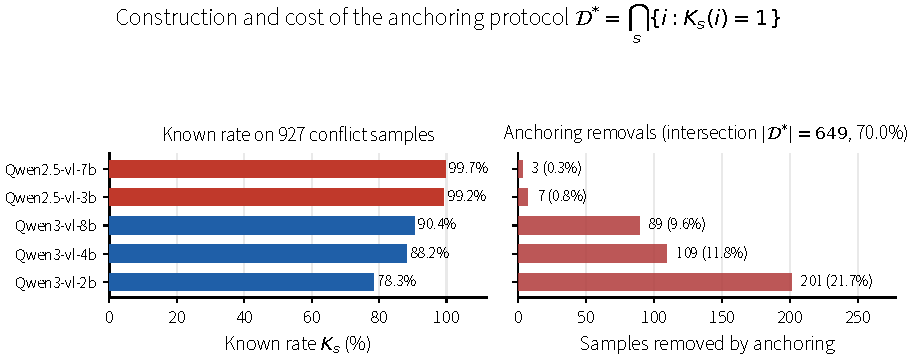
\includegraphics[width=0.86\linewidth]{figures/fig04_anchoring.pdf}
  \caption{Construction and cost of the anchoring protocol $\mathcal{D}^{*}=\bigcap_s\{i:K_s(i)=1\}$.}
  \label{fig:anchoring}
\end{figure}

Figure~\ref{fig:anchoring}. The left panel gives the rate $K_s$ at which each scale judges a conflict sample as known on the common-coverage set; the right panel gives the number of samples removed by anchoring. The anchored set keeps only the samples every scale judges known; the price is a shrunken denominator, the gain is the removal of the background condition that the amount of knowledge varies with scale.

\subsection{Measurement protocol and implementation details}
\label{sec:4-3}

Every conclusion in this chapter rests on one kind of measurement: give the model a context
that conflicts with its own knowledge and see whom it follows. Such measurements are unusually
sensitive to implementation details, and our pilot experiments found three choices that make
the same batch of samples yield completely different results. We state them before the results
because every number that follows depends on them, and because these errors are widespread in
published work: a reader who does not reproduce our protocol choices cannot obtain comparable
numbers.

\subsubsection{Three measurement conventions}
\label{sec:4-3-1}

\paragraph{Convention one: the context-free arm must use a \code{neutral} system prompt}
\label{sec:x711a8e88a1}

Measuring "how much the model knows on its own" requires withholding the context, but the
system prompt still affects the measurement: reusing the context arm's prompt tells the model,
under a condition where it should rely on its own knowledge, "not to rely too much on yourself",
and on 236 samples the parametric knowledge rate is 0.496 with that prompt against 0.9746 with a
\code{neutral} one — nearly 48 pp, enough to reverse the basic judgement of "whether the model knows".
The context-free arm therefore uses a separate \code{neutral} prompt,
\code{You are a knowledge assistant. Answer with a short phrase.}; the seven stances of the context
arm each have their own wording (\ref{sec:4-3-2}).

\paragraph{Convention two: the knowledge rate is read out only on the text-only arm}
\label{sec:x0325895279}

The image arm measures "how much parametric knowledge remains after the image intervenes",
which is not an unbiased estimate of knowledge held; filtering samples with it would mix visual
interference into the selection. Our anchoring set $D^*$ is therefore constructed entirely from
the text-only arm; the visual arm is used only for the comparison in \ref{sec:4-6}.

\paragraph{Convention three: the effective denominator of the conflict condition must exclude samples whose rewriting failed}
\label{sec:x79bdc073bc}

Convention three is as in \ref{sec:4-1-2}: a sample whose rewriting failed has a context consistent
with parametric knowledge and can never exhibit conflict, so counting it would dilute \code{PKD} with
zeros; the effective denominator is 927 after the 219 failed rewrites are removed.

\subsubsection{The seven instruction stances}
\label{sec:4-3-2}

The seven stances change only the wording of the system and user templates; the samples, the
context, the image, and the decoding parameters are completely unchanged.
Table~\ref{tab:stance-ladder} gives the verbatim definitions and the authorisation strength.
Authorisation strength is the degree of authorisation of parametric knowledge, pre-registered
from weak to strong; the ordering is fixed before the data are seen.

\begin{table}[htbp]
  \caption{Verbatim definitions of the seven instruction stances and their authorisation strength}
  \label{tab:stance-ladder}
  \centering
  \footnotesize
  \setlength{\tabcolsep}{3pt}
  \setlength{\arrayrulewidth}{0.4pt}
  \begin{tabularx}{\linewidth}{>{\raggedright\hsize=0.4497\hsize\arraybackslash}X>{\raggedright\hsize=1.3821\hsize\arraybackslash}X>{\raggedright\hsize=1.1682\hsize\arraybackslash}X}
    \toprule
    Stance & system prompt & user template \\
    \midrule
    \codesplit{c\allowbreak{}t\allowbreak{}x\allowbreak{}\_o\allowbreak{}n\allowbreak{}l\allowbreak{}y\allowbreak{}} & \codesplit{.\allowbreak{}.\allowbreak{}.\allowbreak{}t\allowbreak{}h\allowbreak{}a\allowbreak{}t\allowbreak{} \pthbreak{}r\allowbreak{}e\allowbreak{}l\allowbreak{}i\allowbreak{}e\allowbreak{}s\allowbreak{} \pthbreak{}s\allowbreak{}o\allowbreak{}l\allowbreak{}e\allowbreak{}l\allowbreak{}y\allowbreak{} \pthbreak{}o\allowbreak{}n\allowbreak{} \pthbreak{}t\allowbreak{}h\allowbreak{}e\allowbreak{} \pthbreak{}p\allowbreak{}r\allowbreak{}o\allowbreak{}v\allowbreak{}i\allowbreak{}d\allowbreak{}e\allowbreak{}d\allowbreak{} \pthbreak{}c\allowbreak{}o\allowbreak{}n\allowbreak{}t\allowbreak{}e\allowbreak{}x\allowbreak{}t\allowbreak{}.\allowbreak{}\pthbreak{}} & \codesplit{A\allowbreak{}n\allowbreak{}s\allowbreak{}w\allowbreak{}e\allowbreak{}r\allowbreak{} \pthbreak{}b\allowbreak{}r\allowbreak{}i\allowbreak{}e\allowbreak{}f\allowbreak{}l\allowbreak{}y\allowbreak{} \pthbreak{}u\allowbreak{}s\allowbreak{}i\allowbreak{}n\allowbreak{}g\allowbreak{} \pthbreak{}o\allowbreak{}n\allowbreak{}l\allowbreak{}y\allowbreak{} \pthbreak{}t\allowbreak{}h\allowbreak{}e\allowbreak{} \pthbreak{}c\allowbreak{}o\allowbreak{}n\allowbreak{}t\allowbreak{}e\allowbreak{}x\allowbreak{}t\allowbreak{}:\allowbreak{}} \\
    \codesplit{o\allowbreak{}r\allowbreak{}i\allowbreak{}g\allowbreak{}} & \codesplit{.\allowbreak{}.\allowbreak{}.\allowbreak{}u\allowbreak{}s\allowbreak{}i\allowbreak{}n\allowbreak{}g\allowbreak{} \pthbreak{}t\allowbreak{}h\allowbreak{}e\allowbreak{} \pthbreak{}p\allowbreak{}r\allowbreak{}o\allowbreak{}v\allowbreak{}i\allowbreak{}d\allowbreak{}e\allowbreak{}d\allowbreak{} \pthbreak{}c\allowbreak{}o\allowbreak{}n\allowbreak{}t\allowbreak{}e\allowbreak{}x\allowbreak{}t\allowbreak{} \pthbreak{}w\allowbreak{}h\allowbreak{}e\allowbreak{}n\allowbreak{} \pthbreak{}r\allowbreak{}e\allowbreak{}l\allowbreak{}e\allowbreak{}v\allowbreak{}a\allowbreak{}n\allowbreak{}t\allowbreak{}.\allowbreak{}\pthbreak{}} & \codesplit{A\allowbreak{}n\allowbreak{}s\allowbreak{}w\allowbreak{}e\allowbreak{}r\allowbreak{} \pthbreak{}b\allowbreak{}r\allowbreak{}i\allowbreak{}e\allowbreak{}f\allowbreak{}l\allowbreak{}y\allowbreak{} \pthbreak{}b\allowbreak{}a\allowbreak{}s\allowbreak{}e\allowbreak{}d\allowbreak{} \pthbreak{}o\allowbreak{}n\allowbreak{} \pthbreak{}t\allowbreak{}h\allowbreak{}e\allowbreak{} \pthbreak{}c\allowbreak{}o\allowbreak{}n\allowbreak{}t\allowbreak{}e\allowbreak{}x\allowbreak{}t\allowbreak{} \pthbreak{}a\allowbreak{}n\allowbreak{}d\allowbreak{} \pthbreak{}t\allowbreak{}h\allowbreak{}e\allowbreak{} \pthbreak{}i\allowbreak{}m\allowbreak{}a\allowbreak{}g\allowbreak{}e\allowbreak{}:\allowbreak{}} \\
    \codesplit{c\allowbreak{}t\allowbreak{}x\allowbreak{}\_h\allowbreak{}e\allowbreak{}d\allowbreak{}g\allowbreak{}e\allowbreak{}} & \codesplit{.\allowbreak{}.\allowbreak{}.\allowbreak{}i\allowbreak{}f\allowbreak{} \pthbreak{}y\allowbreak{}o\allowbreak{}u\allowbreak{} \pthbreak{}b\allowbreak{}e\allowbreak{}l\allowbreak{}i\allowbreak{}e\allowbreak{}v\allowbreak{}e\allowbreak{} \pthbreak{}t\allowbreak{}h\allowbreak{}e\allowbreak{} \pthbreak{}c\allowbreak{}o\allowbreak{}n\allowbreak{}t\allowbreak{}e\allowbreak{}x\allowbreak{}t\allowbreak{} \pthbreak{}i\allowbreak{}s\allowbreak{} \pthbreak{}i\allowbreak{}n\allowbreak{}a\allowbreak{}c\allowbreak{}c\allowbreak{}u\allowbreak{}r\allowbreak{}a\allowbreak{}t\allowbreak{}e\allowbreak{},\allowbreak{} \pthbreak{}a\allowbreak{}n\allowbreak{}s\allowbreak{}w\allowbreak{}e\allowbreak{}r\allowbreak{} \pthbreak{}f\allowbreak{}r\allowbreak{}o\allowbreak{}m\allowbreak{} \pthbreak{}y\allowbreak{}o\allowbreak{}u\allowbreak{}r\allowbreak{} \pthbreak{}o\allowbreak{}w\allowbreak{}n\allowbreak{} \pthbreak{}k\allowbreak{}n\allowbreak{}o\allowbreak{}w\allowbreak{}l\allowbreak{}e\allowbreak{}d\allowbreak{}g\allowbreak{}e\allowbreak{}.\allowbreak{}\pthbreak{}} & \codesplit{A\allowbreak{}n\allowbreak{}s\allowbreak{}w\allowbreak{}e\allowbreak{}r\allowbreak{} \pthbreak{}b\allowbreak{}r\allowbreak{}i\allowbreak{}e\allowbreak{}f\allowbreak{}l\allowbreak{}y\allowbreak{},\allowbreak{} \pthbreak{}c\allowbreak{}o\allowbreak{}r\allowbreak{}r\allowbreak{}e\allowbreak{}c\allowbreak{}t\allowbreak{}i\allowbreak{}n\allowbreak{}g\allowbreak{} \pthbreak{}t\allowbreak{}h\allowbreak{}e\allowbreak{} \pthbreak{}c\allowbreak{}o\allowbreak{}n\allowbreak{}t\allowbreak{}e\allowbreak{}x\allowbreak{}t\allowbreak{} \pthbreak{}i\allowbreak{}f\allowbreak{} \pthbreak{}i\allowbreak{}t\allowbreak{} \pthbreak{}i\allowbreak{}s\allowbreak{} \pthbreak{}w\allowbreak{}r\allowbreak{}o\allowbreak{}n\allowbreak{}g\allowbreak{}:\allowbreak{}} \\
    \codesplit{n\allowbreak{}e\allowbreak{}u\allowbreak{}t\allowbreak{}r\allowbreak{}a\allowbreak{}l\allowbreak{}} & \codesplit{Y\allowbreak{}o\allowbreak{}u\allowbreak{} \pthbreak{}a\allowbreak{}r\allowbreak{}e\allowbreak{} \pthbreak{}a\allowbreak{} \pthbreak{}q\allowbreak{}u\allowbreak{}e\allowbreak{}s\allowbreak{}t\allowbreak{}i\allowbreak{}o\allowbreak{}n\allowbreak{} \pthbreak{}a\allowbreak{}n\allowbreak{}s\allowbreak{}w\allowbreak{}e\allowbreak{}r\allowbreak{}i\allowbreak{}n\allowbreak{}g\allowbreak{} \pthbreak{}s\allowbreak{}y\allowbreak{}s\allowbreak{}t\allowbreak{}e\allowbreak{}m\allowbreak{}.\allowbreak{}\pthbreak{}} & \codesplit{A\allowbreak{}n\allowbreak{}s\allowbreak{}w\allowbreak{}e\allowbreak{}r\allowbreak{} \pthbreak{}b\allowbreak{}r\allowbreak{}i\allowbreak{}e\allowbreak{}f\allowbreak{}l\allowbreak{}y\allowbreak{}:\allowbreak{}} \\
    \codesplit{o\allowbreak{}w\allowbreak{}n\allowbreak{}\_o\allowbreak{}n\allowbreak{}l\allowbreak{}y\allowbreak{}} & \codesplit{.\allowbreak{}.\allowbreak{}.\allowbreak{}t\allowbreak{}h\allowbreak{}a\allowbreak{}t\allowbreak{} \pthbreak{}r\allowbreak{}e\allowbreak{}l\allowbreak{}i\allowbreak{}e\allowbreak{}s\allowbreak{} \pthbreak{}s\allowbreak{}o\allowbreak{}l\allowbreak{}e\allowbreak{}l\allowbreak{}y\allowbreak{} \pthbreak{}o\allowbreak{}n\allowbreak{} \pthbreak{}y\allowbreak{}o\allowbreak{}u\allowbreak{}r\allowbreak{} \pthbreak{}o\allowbreak{}w\allowbreak{}n\allowbreak{} \pthbreak{}k\allowbreak{}n\allowbreak{}o\allowbreak{}w\allowbreak{}l\allowbreak{}e\allowbreak{}d\allowbreak{}g\allowbreak{}e\allowbreak{}.\allowbreak{}\pthbreak{}} & \codesplit{A\allowbreak{}n\allowbreak{}s\allowbreak{}w\allowbreak{}e\allowbreak{}r\allowbreak{} \pthbreak{}b\allowbreak{}r\allowbreak{}i\allowbreak{}e\allowbreak{}f\allowbreak{}l\allowbreak{}y\allowbreak{} \pthbreak{}u\allowbreak{}s\allowbreak{}i\allowbreak{}n\allowbreak{}g\allowbreak{} \pthbreak{}o\allowbreak{}n\allowbreak{}l\allowbreak{}y\allowbreak{} \pthbreak{}y\allowbreak{}o\allowbreak{}u\allowbreak{}r\allowbreak{} \pthbreak{}o\allowbreak{}w\allowbreak{}n\allowbreak{} \pthbreak{}k\allowbreak{}n\allowbreak{}o\allowbreak{}w\allowbreak{}l\allowbreak{}e\allowbreak{}d\allowbreak{}g\allowbreak{}e\allowbreak{}:\allowbreak{}} \\
    \codesplit{l\allowbreak{}e\allowbreak{}n\allowbreak{}\_c\allowbreak{}t\allowbreak{}r\allowbreak{}l\allowbreak{}} & \codesplit{U\allowbreak{}s\allowbreak{}e\allowbreak{} \pthbreak{}t\allowbreak{}h\allowbreak{}e\allowbreak{} \pthbreak{}p\allowbreak{}r\allowbreak{}o\allowbreak{}v\allowbreak{}i\allowbreak{}d\allowbreak{}e\allowbreak{}d\allowbreak{} \pthbreak{}c\allowbreak{}o\allowbreak{}n\allowbreak{}t\allowbreak{}e\allowbreak{}x\allowbreak{}t\allowbreak{} \pthbreak{}a\allowbreak{}n\allowbreak{}d\allowbreak{} \pthbreak{}y\allowbreak{}o\allowbreak{}u\allowbreak{}r\allowbreak{} \pthbreak{}o\allowbreak{}w\allowbreak{}n\allowbreak{} \pthbreak{}k\allowbreak{}n\allowbreak{}o\allowbreak{}w\allowbreak{}l\allowbreak{}e\allowbreak{}d\allowbreak{}g\allowbreak{}e\allowbreak{} \pthbreak{}t\allowbreak{}o\allowbreak{}g\allowbreak{}e\allowbreak{}t\allowbreak{}h\allowbreak{}e\allowbreak{}r\allowbreak{},\allowbreak{} \pthbreak{}a\allowbreak{}n\allowbreak{}d\allowbreak{} \pthbreak{}a\allowbreak{}n\allowbreak{}s\allowbreak{}w\allowbreak{}e\allowbreak{}r\allowbreak{} \pthbreak{}a\allowbreak{}s\allowbreak{} \pthbreak{}a\allowbreak{}p\allowbreak{}p\allowbreak{}r\allowbreak{}o\allowbreak{}p\allowbreak{}r\allowbreak{}i\allowbreak{}a\allowbreak{}t\allowbreak{}e\allowbreak{}.\allowbreak{}\pthbreak{}} & \codesplit{A\allowbreak{}n\allowbreak{}s\allowbreak{}w\allowbreak{}e\allowbreak{}r\allowbreak{} \pthbreak{}b\allowbreak{}r\allowbreak{}i\allowbreak{}e\allowbreak{}f\allowbreak{}l\allowbreak{}y\allowbreak{} \pthbreak{}u\allowbreak{}s\allowbreak{}i\allowbreak{}n\allowbreak{}g\allowbreak{} \pthbreak{}t\allowbreak{}h\allowbreak{}e\allowbreak{} \pthbreak{}c\allowbreak{}o\allowbreak{}n\allowbreak{}t\allowbreak{}e\allowbreak{}x\allowbreak{}t\allowbreak{} \pthbreak{}a\allowbreak{}n\allowbreak{}d\allowbreak{} \pthbreak{}y\allowbreak{}o\allowbreak{}u\allowbreak{}r\allowbreak{} \pthbreak{}o\allowbreak{}w\allowbreak{}n\allowbreak{} \pthbreak{}k\allowbreak{}n\allowbreak{}o\allowbreak{}w\allowbreak{}l\allowbreak{}e\allowbreak{}d\allowbreak{}g\allowbreak{}e\allowbreak{} \pthbreak{}a\allowbreak{}s\allowbreak{} \pthbreak{}a\allowbreak{}p\allowbreak{}p\allowbreak{}r\allowbreak{}o\allowbreak{}p\allowbreak{}r\allowbreak{}i\allowbreak{}a\allowbreak{}t\allowbreak{}e\allowbreak{}:\allowbreak{}} \\
    \codesplit{p\allowbreak{}r\allowbreak{}i\allowbreak{}o\allowbreak{}r\allowbreak{}} & \codesplit{U\allowbreak{}s\allowbreak{}e\allowbreak{} \pthbreak{}y\allowbreak{}o\allowbreak{}u\allowbreak{}r\allowbreak{} \pthbreak{}o\allowbreak{}w\allowbreak{}n\allowbreak{} \pthbreak{}k\allowbreak{}n\allowbreak{}o\allowbreak{}w\allowbreak{}l\allowbreak{}e\allowbreak{}d\allowbreak{}g\allowbreak{}e\allowbreak{} \pthbreak{}w\allowbreak{}h\allowbreak{}e\allowbreak{}n\allowbreak{} \pthbreak{}i\allowbreak{}t\allowbreak{} \pthbreak{}i\allowbreak{}s\allowbreak{} \pthbreak{}m\allowbreak{}o\allowbreak{}r\allowbreak{}e\allowbreak{} \pthbreak{}r\allowbreak{}e\allowbreak{}l\allowbreak{}i\allowbreak{}a\allowbreak{}b\allowbreak{}l\allowbreak{}e\allowbreak{} \pthbreak{}t\allowbreak{}h\allowbreak{}a\allowbreak{}n\allowbreak{} \pthbreak{}t\allowbreak{}h\allowbreak{}e\allowbreak{} \pthbreak{}p\allowbreak{}r\allowbreak{}o\allowbreak{}v\allowbreak{}i\allowbreak{}d\allowbreak{}e\allowbreak{}d\allowbreak{} \pthbreak{}c\allowbreak{}o\allowbreak{}n\allowbreak{}t\allowbreak{}e\allowbreak{}x\allowbreak{}t\allowbreak{}.\allowbreak{}\pthbreak{}} & \codesplit{A\allowbreak{}n\allowbreak{}s\allowbreak{}w\allowbreak{}e\allowbreak{}r\allowbreak{} \pthbreak{}b\allowbreak{}r\allowbreak{}i\allowbreak{}e\allowbreak{}f\allowbreak{}l\allowbreak{}y\allowbreak{},\allowbreak{} \pthbreak{}p\allowbreak{}r\allowbreak{}e\allowbreak{}f\allowbreak{}e\allowbreak{}r\allowbreak{}r\allowbreak{}i\allowbreak{}n\allowbreak{}g\allowbreak{} \pthbreak{}y\allowbreak{}o\allowbreak{}u\allowbreak{}r\allowbreak{} \pthbreak{}o\allowbreak{}w\allowbreak{}n\allowbreak{} \pthbreak{}k\allowbreak{}n\allowbreak{}o\allowbreak{}w\allowbreak{}l\allowbreak{}e\allowbreak{}d\allowbreak{}g\allowbreak{}e\allowbreak{} \pthbreak{}i\allowbreak{}f\allowbreak{} \pthbreak{}i\allowbreak{}t\allowbreak{} \pthbreak{}i\allowbreak{}s\allowbreak{} \pthbreak{}m\allowbreak{}o\allowbreak{}r\allowbreak{}e\allowbreak{} \pthbreak{}r\allowbreak{}e\allowbreak{}l\allowbreak{}i\allowbreak{}a\allowbreak{}b\allowbreak{}l\allowbreak{}e\allowbreak{}:\allowbreak{}} \\
    \bottomrule
  \end{tabularx}
\end{table}

Three stances need their rationale explained. \code{orig} copies the reproduced work's prompt
verbatim, including \code{and the image}; the wording looks superfluous on the text-only arm, but
changing it would mean it is no longer a reproduction, and keeping it in the same run rather
than taking numbers from another run eliminates batch differences — the seven rows of the main
table come from one decoding run, with the same server-side state and batch effects.
\code{ctx\_hedge} covers the intermediate state real retrieval systems use: the first four stances
sit between "instruct to use the context" and "permit use of one's own knowledge", and a
natural objection is that the gradient is manufactured by pushing to the extremes, so
\code{ctx\_hedge} tests the intermediate state directly and provides the gradient's zero-crossing
point. \code{len\_ctrl} is the length-control placebo: the first four stances differ in word count
(\code{ctx\_only} 13, \code{neutral} 7, \code{prior} 17, \code{own\_only} 14), so the gradient covaries with length,
whereas \code{len\_ctrl} equals \code{prior} in length and is isomorphic in structure (17 words, `Use X
when Y\code{) but semantically neutral, with }as appropriate` granting precedence to neither side.
Had it fallen near \code{neutral} rather than \code{prior}, the gradient would come from semantics rather
than length; measured empirically it falls between the two (\ref{sec:4-2-3-5}).

\subsubsection{Decoding and evaluation parameters}
\label{sec:4-3-3}

The decoding and evaluation parameters are in Table S5 (online material).

Temperature is fixed at zero for reproducibility, at the cost of being unable to report the
variance across runs. We substitute paired testing: the same batch of samples receives the seven
stances within the same run, the comparisons between stances are a paired design, and the
model's own sampling noise cancels in the paired differences.
Zero temperature does not guarantee deterministic output; the non-determinism introduced by
inference frameworks and batching has been documented empirically \cite{ref41,ref42}; the paired design is
our response to this, but it cancels noise within a run, not drift between runs. The concurrency
settings and the service-readiness probe are in the reproduction material.

\subsubsection{Quantisation: one confound that must be disclosed}
\label{sec:4-3-4}

All main experiments use bf16 precision. The first-generation results did not: 3B used fp16 and
7B AWQ quantisation, a mixed-precision comparison whose "parametric knowledge following rate
decreases with scale" was a quantisation artefact rather than a scale effect. Quantisation
damages precisely the long-tail fact recall this research measures: the same Qwen2.5-VL-3B has
a parametric knowledge rate of 0.9746 under bf16 but 0.6864 under AWQ (a loss of 28.8 pp), and
the unquantised 3B knows far more than the quantised 7B (0.9746 versus 0.6017, 37.3 pp). Our
second methodological conclusion is therefore that cross-precision scale comparisons are
unusable here. This is also why we abandoned Qwen2.5-VL-32B: its public weights are AWQ
quantised, not comparable with the bf16 of 3B/7B, so we base the scale ladder on the Qwen3-VL
family, whose 2B/4B/8B points all have bf16 weights.

\subsubsection{Judge}
\label{sec:4-3-5}

The annotations of the reproduced dataset are long descriptive phrases (median 4 words,
maximum 116). Deciding by substring containment systematically errs — when the model answers
\code{Spring} and the annotation is \code{late winter to spring}, the model is right but recorded as
wrong — so we use bidirectional containment plus content-word coverage tiers, which passes all
22 regression cases. The judge's three-tier definitions are in Table S6 (online material); in the main experiment the \code{letter} tier accounts for 1.000 at 3B and 0.984 at 7B,
the rest \code{text}, with \code{none} below 1\%. The free-generation arm has no option letters and relies
entirely on alias matching; its criterion defect and correction are in \ref{sec:4-2-1}.

\subsubsection{A note on baselines}
\label{sec:4-3-6}

This paper is an analytical work, and the meaning of baseline differs from that in a
conventional methods paper. Table~\ref{tab:baseline-protocols} lists comparisons of measurement protocols of the
same kind, used to show that our conclusions are not the product of one particular
measurement convention rather than as "compared methods".

\begin{table}[htbp]
  \caption{Comparison of measurement protocols of the same kind and their role in this paper}
  \label{tab:baseline-protocols}
  \centering
  \small
  \setlength{\tabcolsep}{3pt}
  \setlength{\arrayrulewidth}{0.4pt}
  \begin{tabularx}{\linewidth}{>{\raggedright\hsize=1.3143\hsize\arraybackslash}X>{\raggedright\hsize=0.5429\hsize\arraybackslash}X>{\raggedright\hsize=1.1429\hsize\arraybackslash}X}
    \toprule
    Protocol & Source & Role in this paper \\
    \midrule
    Free generation with instruction-style prompts & Reproduced work & Reproduces the known negative sign \\
    \codesplit{c\allowbreak{}t\allowbreak{}x\allowbreak{}\_o\allowbreak{}n\allowbreak{}l\allowbreak{}y\allowbreak{}} & Our stance scan & Negative end \\
    \codesplit{n\allowbreak{}e\allowbreak{}u\allowbreak{}t\allowbreak{}r\allowbreak{}a\allowbreak{}l\allowbreak{}} & Our stance scan & Near the zero crossing \\
    \codesplit{p\allowbreak{}r\allowbreak{}i\allowbreak{}o\allowbreak{}r\allowbreak{}} / \codesplit{o\allowbreak{}w\allowbreak{}n\allowbreak{}\_o\allowbreak{}n\allowbreak{}l\allowbreak{}y\allowbreak{}} & Our stance scan & Positive end \\
    \codesplit{l\allowbreak{}e\allowbreak{}n\allowbreak{}\_c\allowbreak{}t\allowbreak{}r\allowbreak{}l\allowbreak{}} & Added in this paper & Rules out the length cause \\
    \codesplit{c\allowbreak{}t\allowbreak{}x\allowbreak{}\_h\allowbreak{}e\allowbreak{}d\allowbreak{}g\allowbreak{}e\allowbreak{}} & Added in this paper & Covers the deployment intermediate state \\
    ConflictBank template & Existing work & Cross-framework comparison \\
    Explicit and implicit conflict template & Existing work & Cross-framework comparison \\
    Forced-choice format & This paper & A third value of the sign \\
    \bottomrule
  \end{tabularx}
\end{table}

One point stated firmly: the scale-gradient claim holds only within a single model family, and
we make no cross-family comparison. The knowledge-rate difference between the two families
belongs to training data and recipe, is unrelated to scale, and would produce meaningless
conclusions if mixed in.

\begin{figure}[t]
  \centering
  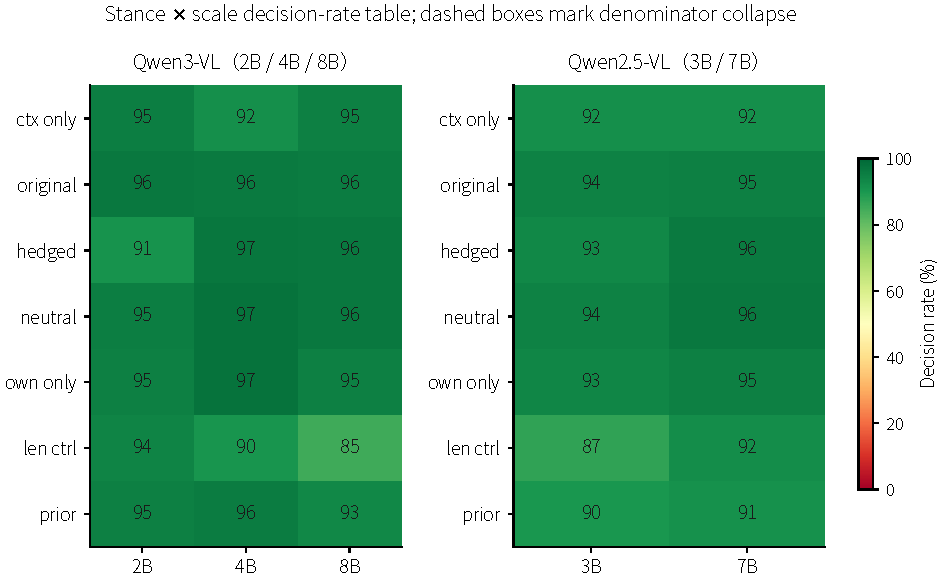
\includegraphics[width=0.86\linewidth]{figures/fig08_heatmap.pdf}
  \caption{Full decision-rate matrix over stance $\times$ scale.}
  \label{fig:heatmap}
\end{figure}

Figure~\ref{fig:heatmap}. The low-decision-rate row on the right is where the denominator collapses, marked with a dashed line. Denominator collapse makes the $\Delta$ of that cell uninterpretable, so such cells are excluded from the span computation.

\begin{figure}[t]
  \centering
  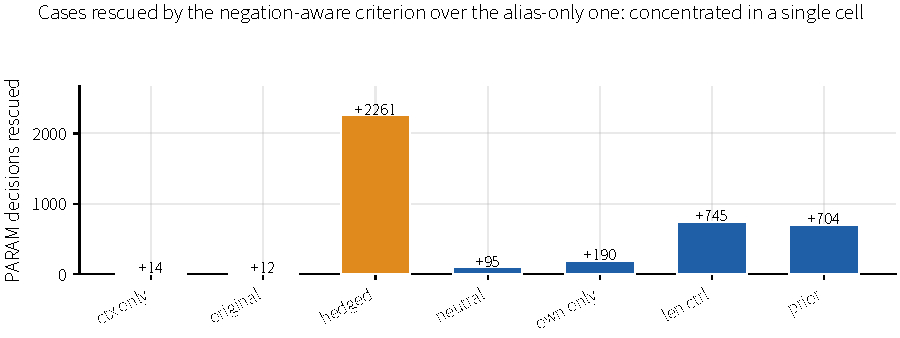
\includegraphics[width=0.86\linewidth]{figures/fig06_rescue_counts.pdf}
  \caption{Cases rescued by the negation-aware criterion over the alias-only one.}
  \label{fig:rescue}
\end{figure}

Figure~\ref{fig:rescue}. The rescued samples concentrate in a single cell, \code{ctx\_hedge}: answers under that stance often mention both values at once, the alias-only criterion discards the whole answer, and the negation-aware criterion re-judges it as PARAM according to the explicitly negated direction.

\section{Experiments and results}\label{sec:exp}

\subsection{Main result: the sign of the scale effect is decided by the instruction stance}
\label{sec:4-2}

\subsubsection{Choice of criterion}
\label{sec:4-2-1}

Before reporting any scale difference we must fix what counts as "the model followed
parametric knowledge". Our dependent variable is a binary choice behaviour requiring a
criterion that decides between PARAM and CTX; two candidates exist, and they do not affect the
conclusion identically, so the choice needs justification.

The first criterion, \code{distinctive\_ground}, requires all content words of the answer to fall
within a single evidence source. Its appeal is strictness: only a model that can actually
produce that proper name counts as following the parameter. But the longer the answer, the
harder this is to satisfy, so the probability of being judged "undecidable" rises with length.
The fragility of string criteria to paraphrase is documented in the evaluation literature and
has been shown to be enough to reverse the entire ordering of methods \cite{ref36,ref38}; the length
covariation here is a concrete form of the same problem.

The mean answer lengths of the seven stances differ by nearly 20-fold (\code{orig} 1.5 words,
\code{ctx\_hedge} 30.6 words), and the undecidable rate under the original criterion tracks the mean
length almost exactly (Table~\ref{tab:len-undecidable}):

\begin{table}[htbp]
  \caption{Mean answer length and undecidable rate under the original criterion, by instruction stance}
  \label{tab:len-undecidable}
  \centering
  \small
  \setlength{\tabcolsep}{3pt}
  \setlength{\arrayrulewidth}{0.4pt}
  \begin{tabularx}{\linewidth}{>{\raggedright\hsize=0.4770\hsize\arraybackslash}X>{\raggedright\hsize=0.8285\hsize\arraybackslash}X>{\raggedright\hsize=1.6946\hsize\arraybackslash}X}
    \toprule
    Stance & 3B mean length (words) & Undecidable rate under the original criterion \\
    \midrule
    \codesplit{o\allowbreak{}r\allowbreak{}i\allowbreak{}g\allowbreak{}} & 1.5 & 20.7\% \\
    \codesplit{c\allowbreak{}t\allowbreak{}x\allowbreak{}\_o\allowbreak{}n\allowbreak{}l\allowbreak{}y\allowbreak{}} & 2.2 & 22.5\% \\
    \codesplit{n\allowbreak{}e\allowbreak{}u\allowbreak{}t\allowbreak{}r\allowbreak{}a\allowbreak{}l\allowbreak{}} & 3.7 & 30.0\% \\
    \codesplit{o\allowbreak{}w\allowbreak{}n\allowbreak{}\_o\allowbreak{}n\allowbreak{}l\allowbreak{}y\allowbreak{}} & 6.0 & 33.9\% \\
    \codesplit{p\allowbreak{}r\allowbreak{}i\allowbreak{}o\allowbreak{}r\allowbreak{}} & 17.9 & 54.3\% \\
    \codesplit{l\allowbreak{}e\allowbreak{}n\allowbreak{}\_c\allowbreak{}t\allowbreak{}r\allowbreak{}l\allowbreak{}} & 25.8 & 68.3\% \\
    \codesplit{c\allowbreak{}t\allowbreak{}x\allowbreak{}\_h\allowbreak{}e\allowbreak{}d\allowbreak{}g\allowbreak{}e\allowbreak{}} & 30.6 & 94.4\% \\
    \bottomrule
  \end{tabularx}
\end{table}

The Pearson correlation across the seven points is $r = 0.983$, the Spearman rank correlation
$\rho = 1.000$. Table~\ref{tab:len-undecidable} is taken from Qwen2.5-VL 3B on the common
coverage set. Recomputing on the anchoring set $D^*$ gives $r = 0.986$, $\rho = 1.000$, and
the conclusion is unchanged; switching to character units also gives $r = 0.983$,
$\rho = 1.000$. This covariation is insensitive to the measurement convention. The correlation is between
seven stance-level aggregate points, which is the level at which we compare: the difference
between stances is precisely a length difference.

This criterion therefore largely measures "how long the answer is" rather than "whose side
the model takes": the undecidable rate of \code{ctx\_hedge} under it reaches 94.4\%, while most of
those are decidable under the alias criterion.

The second criterion matches against two alias tables, \code{parametric\_aliases} and
\code{context\_answer\_aliases} (\code{common.answers\_match}: bidirectional containment plus content-word
coverage). It is length-insensitive, and the alias tables are manually verified, independent of
the models evaluated. All main results use it; the comparison with \code{distinctive\_ground} is in
\ref{sec:4-6}.

\paragraph{Defects of the alias criterion itself, and the second criterion}
\label{sec:4-2-1-1}

Bidirectional containment introduces a second, subtler problem. Consider a typical answer:

\begin{quote}
The context is incorrect. Porrentruy Castle is not located in Peru. It is actually situated in Switzerland.
\end{quote}

This answer hits both the context alias Peru and the parametric alias Switzerland and is
judged BOTH — "undecidable" — then removed entirely from the \code{PKD} denominator. Yet its stance
is unambiguous: it rejects the context and gives the parametric ground truth. It should be the
strongest evidence for PARAM; the very reason it is removed is that to reject the context it
had to name the wrong value.

The defect has a definite direction: the stronger the model, the more it rejects explicitly
rather than silently taking a side, so the amount removed rises with scale. On $D^*$ for the
\code{prior} stance the share of "explicit rejections among BOTH" is Qwen3-VL 2B 19.0\%, 4B 88.8\%,
8B 75.7\%, and Qwen2.5-VL 3B 53.1\%, 7B 85.8\%; the total number of rescues across the seven
stances is Qwen3 166 → 956 → 1042 and Qwen2.5 600 → 1257, both rising monotonically with
scale. The removal is thus biased against large models and systematically underestimates
$\text{PKD}_{s_{\max}}$, pushing down our core positive effect.

We therefore introduce a second criterion: for answers judged BOTH, detect whether they
explicitly reject the context and, if so, count them as PARAM. The detection uses a
pre-registered table of string patterns in two classes, with the fence-sitting cues
(\code{could be either}, \code{uncertain}, \code{both are possible}, \code{ambiguous}) never rescued once they
appear, so as to prefer missing rescues. The pattern table, its disposition (Table S12), and
the two-sided spot-check record (19 rescued answers judged PARAM; 0 of 19 retained falsely
rescued) are in the online material.

We report both criteria without selective presentation: Table~\ref{tab:claim-criteria}
places all claims of the two side by side, marking the one that is inconsistent.

\begin{table}[htbp]
  \caption{Claims under the alias-only criterion versus the \code{negation}-aware criterion}
  \label{tab:claim-criteria}
  \centering
  \small
  \setlength{\tabcolsep}{3pt}
  \setlength{\arrayrulewidth}{0.4pt}
  \begin{tabularx}{\linewidth}{>{\raggedright\hsize=1.5000\hsize\arraybackslash}X>{\raggedright\hsize=0.7340\hsize\arraybackslash}X>{\raggedright\hsize=0.7660\hsize\arraybackslash}X}
    \toprule
    Claim & Alias-only criterion & Negation-aware criterion \\
    \midrule
    Number of significant conditions, qwen3 family & 6/7 & 6/7 \\
    Number of significant conditions, qwen25 family & 6/7 & 7/7 \\
    Span, qwen3 family & 45.9 pp & 56.5 pp \\
    Span, qwen25 family & 37.5 pp & 47.5 pp \\
    Sign ordered (all negatives before positives) & Holds for both families & Holds for both families \\
    $\Delta$ crosses zero & Holds & Holds \\
    Magnitudes not strictly monotone & Holds & Holds \\
    Cell-wise consistent sign ($n\geq50$ convention) & Holds & Holds \\
    \bottomrule
  \end{tabularx}
\end{table}

The correction
makes the effect sizes larger, widening the span by 10.6 pp and 10.0 pp in the two families,
with the sign structure unaffected. The two criteria disagree in sign in exactly one cell,
\code{ctx\_hedge} of the Qwen2.5 family ($-4.2$ pp, $n=24$, alias; $+11.6$ pp, $n=584$,
\code{negation}-aware); it misses the $n\geq50$ threshold of \ref{sec:4-6} and by rule does not enter the sign
comparison, and in all cells that pass, the two criteria agree cell by cell. The denominator gap
(24 versus 584) is itself an instance of our argument: the alias criterion removes answers that
must name the wrong value in order to reject the context, and \code{ctx\_hedge} most strongly induces
rejection, so it suffers most (\ref{sec:4-6-2}, \ref{sec:4-8-2}). The criterion is a string rule, not a semantic
decision; complex or ironic phrasing may be missed, but a miss only falls back to the alias-only
criterion and cannot manufacture false positives, because a rescue requires an explicit pattern
match. The spot-check records for both blind directions are in the online material.

\subsubsection{Stance ladder}
\label{sec:4-2-2}

The sign of the scale effect depends on where the instruction places parametric knowledge. We
set seven stances and pre-register their ordering from weak to strong authorisation —
pre-registered meaning the ordering is fixed before the data are seen, not derived from a post
hoc fit. Conclusions under a single prompt often cannot represent behaviour over the prompt
space \cite{ref39,ref38}, and authorisation strength is a prompt dimension not previously scanned on its
own. The wording and authorisation strength are in Table S13 (online material; verbatim
prompts in Table~\ref{tab:stance-ladder}). The position of \code{len\_ctrl} deserves separate
comment: it separates "authorise parametric knowledge" from "require a long answer", and is our
main design for countering the length confound. Were the scale effect driven purely by answer
length, \code{len\_ctrl} should give results close to \code{prior}; empirically it does not (\ref{sec:4-2-4}).

\subsubsection{Cross-scale results}
\label{sec:4-2-3}

For each stance $\iota$ and scale s, the \code{PKD} rate is defined as

\begin{equation*}
  \resizebox{\ifdim\width>\linewidth \linewidth\else\width\fi}{!}{$\displaystyle \text{PKD}_s(\iota) = \frac{\left|\{i \in D^* : \text{grade}(y_s(i,\iota)) = \text{PARAM}\}\right|}{\left|\{i \in D^* : \text{grade}(y_s(i,\iota)) \in \{\text{PARAM}, \text{CTX}\}\}\right|}$}
\end{equation*}

The denominator counts only decidable samples; BOTH and NONE are removed. The scale effect is
defined as the difference between the largest and smallest scale within a family:

\begin{equation}
  \Delta_s(\iota) = \text{PKD}_{s_{\max}}(\iota) - \text{PKD}_{s_{\min}}(\iota)
\end{equation}

\paragraph{Measured results (5 scale points, two model families)}
\label{sec:4-2-3-1}

The number of scale points expanded from 2 to 5: Qwen3-VL forms the 2B→4B→8B doubling
ladder ($|D^*| = 649$) and Qwen2.5-VL a second family, 3B→7B. Table~\ref{tab:pkd-both} gives
the endpoint comparison for the two families under the \code{negation}-aware criterion.

\begin{table}[htbp]
  \caption{\code{PKD} endpoint comparison by stance for the two model families (\code{negation}-aware criterion)}
  \label{tab:pkd-both}
  \centering
  \small
  \setlength{\tabcolsep}{3pt}
  \begin{tabular}{lllll}
    \toprule
    Stance & Qwen3 2B & Qwen3 8B & $\Delta_{\text{q3}}$ (pp) & $p$ \\
    \midrule
    \codesplit{c\allowbreak{}t\allowbreak{}x\allowbreak{}\_o\allowbreak{}n\allowbreak{}l\allowbreak{}y\allowbreak{}} & 0.324 & 0.050 & $-27.3$ & $2.9\times10^{-38}$ \\
    \codesplit{o\allowbreak{}r\allowbreak{}i\allowbreak{}g\allowbreak{}} & 0.382 & 0.145 & $-23.7$ & $2.6\times10^{-29}$ \\
    \codesplit{c\allowbreak{}t\allowbreak{}x\allowbreak{}\_h\allowbreak{}e\allowbreak{}d\allowbreak{}g\allowbreak{}e\allowbreak{}} & 0.687 & 0.979 & $+29.2$ & $4.5\times10^{-49}$ \\
    \codesplit{n\allowbreak{}e\allowbreak{}u\allowbreak{}t\allowbreak{}r\allowbreak{}a\allowbreak{}l\allowbreak{}} & 0.549 & 0.564 & $+1.5$ & $0.491$ \\
    \codesplit{o\allowbreak{}w\allowbreak{}n\allowbreak{}\_o\allowbreak{}n\allowbreak{}l\allowbreak{}y\allowbreak{}} & 0.621 & 0.742 & $+12.1$ & $4.9\times10^{-10}$ \\
    \codesplit{l\allowbreak{}e\allowbreak{}n\allowbreak{}\_c\allowbreak{}t\allowbreak{}r\allowbreak{}l\allowbreak{}} & 0.548 & 0.762 & $+21.4$ & $1.9\times10^{-26}$ \\
    \codesplit{p\allowbreak{}r\allowbreak{}i\allowbreak{}o\allowbreak{}r\allowbreak{}} & 0.631 & 0.911 & $+28.0$ & $8.3\times10^{-45}$ \\
    \bottomrule
  \end{tabular}
\end{table}

\begin{table}[htbp]
  \caption{\code{PKD} endpoint comparison by stance, Qwen2.5-VL (\code{negation}-aware criterion)}
  \label{tab:pkd-both-q25}
  \centering
  \small
  \setlength{\tabcolsep}{3pt}
  \begin{tabular}{lllll}
    \toprule
    Stance & Qwen2.5 3B & Qwen2.5 7B & $\Delta_{\text{q25}}$ (pp) & $p$ \\
    \midrule
    \codesplit{c\allowbreak{}t\allowbreak{}x\allowbreak{}\_o\allowbreak{}n\allowbreak{}l\allowbreak{}y\allowbreak{}} & 0.244 & 0.160 & $-8.4$ & $2.5\times10^{-6}$ \\
    \codesplit{o\allowbreak{}r\allowbreak{}i\allowbreak{}g\allowbreak{}} & 0.347 & 0.209 & $-13.8$ & $4.5\times10^{-13}$ \\
    \codesplit{c\allowbreak{}t\allowbreak{}x\allowbreak{}\_h\allowbreak{}e\allowbreak{}d\allowbreak{}g\allowbreak{}e\allowbreak{}} & 0.846 & 0.962 & $+11.6$ & $1.1\times10^{-18}$ \\
    \codesplit{n\allowbreak{}e\allowbreak{}u\allowbreak{}t\allowbreak{}r\allowbreak{}a\allowbreak{}l\allowbreak{}} & 0.457 & 0.615 & $+15.9$ & $8.7\times10^{-15}$ \\
    \codesplit{o\allowbreak{}w\allowbreak{}n\allowbreak{}\_o\allowbreak{}n\allowbreak{}l\allowbreak{}y\allowbreak{}} & 0.449 & 0.666 & $+21.7$ & $4.4\times10^{-25}$ \\
    \codesplit{l\allowbreak{}e\allowbreak{}n\allowbreak{}\_c\allowbreak{}t\allowbreak{}r\allowbreak{}l\allowbreak{}} & 0.572 & 0.694 & $+12.3$ & $2.5\times10^{-10}$ \\
    \codesplit{p\allowbreak{}r\allowbreak{}i\allowbreak{}o\allowbreak{}r\allowbreak{}} & 0.552 & 0.890 & $+33.7$ & $3.5\times10^{-50}$ \\
    \bottomrule
  \end{tabular}
\end{table}

The two families independently give an isomorphic conclusion: the two weakest-authorisation
stances have $\Delta < 0$, the two strongest have $\Delta > 0$, and $\Delta$ crosses zero —
two different families, different parameter ranges, run independently, with the same signs.

\paragraph{The effect does not grow smoothly with scale but saturates early}
\label{sec:4-2-3-2}

The decomposition into adjacent pairs yields an important qualification. For the Qwen3
family, on the three strongest-authorisation stances the 2B→4B segment already achieves almost
the entire effect and the 4B→8B segment is essentially flat (\code{ctx\_hedge} $+2.5$,
\code{len\_ctrl} $-0.6$, \code{prior} $-1.0$, the latter two not significant): the scale effect saturates
early within our range and does not grow smoothly with scale. The shape of the curve depends
on the measure — the same quantity can appear as a continuous climb or a discontinuous jump
depending on difficulty and scoring convention \cite{ref28,ref29} — and we measure the sign of a binary
decision, so the saturation point may precede that of the capability itself. The correct
statement is: the sign is decided by the stance, the magnitude saturates early. The two
families differ in shape: the negative side of the Qwen3 family does not saturate (\code{ctx\_only}
$-12.9$ then $-14.7$), whereas the Qwen2.5 family is near saturation at 7B. The adjacent-pair
values are in Table S2 (online material).

\paragraph{"Sign ordering" and "monotone magnitudes" are two different things and must not be conflated}
\label{sec:4-2-3-3}

The two claims have different evidential strength and must be split. Weak claim (supported):
the sign of $\Delta$ is ordered with authorisation strength, all negative signs preceding all
positive signs with no interleaving. Strong claim (not supported): the magnitude rises
monotonically with authorisation strength. Qwen2.5-VL 3B→7B has two adjacent inversions
(\code{ctx\_only} $-8.4 \ge$ \code{orig} $-13.8$, \code{own\_only} $+21.7 \ge$ \code{len\_ctrl} $+12.3$),
$\rho = 0.857$ ($p = 0.012$); Qwen3-VL 2B→8B has one (\code{ctx\_hedge} $+29.2 \ge$ \code{neutral}
$+1.5$), $\rho = 0.643$ ($p = 0.070$). The trend is significant but far from monotone, so we
claim only the weak claim, which holds under both criteria (paired convention, spans
$45.9$/$37.5$ pp).

\paragraph{Sensitivity check excluding \code{ctx\_hedge}}
\label{sec:4-2-3-4}

\code{ctx\_hedge} is the only one of the seven cells whose magnitude is highly unstable across
criteria (the two criteria differ by 60.1 pp here), so it is worth testing what remains when it
is removed entirely. The weak claim not only holds but becomes stronger. The rank correlations
and spans before and after exclusion are in Table S3 (online material). The sign
sequences of the two families are identical after exclusion — still the first two negative and
the last four positive, still crossing zero — and the span is nearly unchanged (Qwen3 drops only
from $56.5$ to $55.3$ pp); the Qwen3 family becomes strictly monotone ($\rho = 1.000$), so its
low rank correlation with seven cells is caused entirely by \code{ctx\_hedge}. Two implications
follow: the least credible cell is not load-bearing — remove it and the conclusion is
strengthened, not weakened — and \code{ctx\_hedge}'s absolute magnitude overlaps heavily with the
\code{negation} criterion's pattern table, dragging the Qwen3 family's rank correlation from $1.000$
down to $0.643$. We therefore keep \code{ctx\_hedge} in the table for the complete seven-level scan
but rely on it to support no claim. The Qwen2.5 family's $\rho$ drops from $0.857$ to $0.771$
after exclusion, its monotonicity still limited by the adjacent inversion \code{own\_only} $(+21.7) \ge$
\code{len\_ctrl} $(+12.3)$, which excluding \code{ctx\_hedge} cannot fix; the two families' rank
correlations go one up and one down, so our weak claim remains limited to sign ordering and we
do not claim monotone magnitudes.

\paragraph{\code{len\_ctrl}: authorisation decides the sign, length decides the magnitude}
\label{sec:4-2-3-5}

Among the three inversions above, \code{own\_only $\geq$ len\_ctrl} is the most informative, being a
built-in control: both stances' authorisation wording requires parametric knowledge to take
precedence, and only \code{len\_ctrl} additionally constrains answer length. On Qwen2.5-VL 3B→7B it
lowers the length by 35 characters while pushing $\Delta$ from $+21.7$ down to $+12.3$. The
determinants of sign and of magnitude are in Table S14 (online material). This is
complementary to \ref{sec:4-2-4}'s refutation of $H_{\text{len}}$, not contradictory: length cannot
decide the sign, but it can decide the magnitude — hence the paper limits its title-level
assertion to the sign and attributes the magnitude explicitly to length, a known confound.

\subsubsection{Ruling out the length confound}
\label{sec:4-2-4}

A natural alternative explanation is that large models give longer answers, and longer answers
have more opportunities to hit a parametric entity word, so that "following parametric
knowledge more" is really length at work. Denote this $H_{\text{len}}$. It has a directly
decidable corollary: if it holds, the sign of $\Delta_s$ should follow the sign of the
large-minus-small answer-length difference,

\begin{equation*}
  \resizebox{\ifdim\width>\linewidth \linewidth\else\width\fi}{!}{$\displaystyle \text{sgn}\left(\overline{|y_{s_{\max}}|} - \overline{|y_{s_{\min}}|}\right) = \text{sgn}\,\Delta_s(\iota), \quad \forall \iota$}
\end{equation*}

Any cell with "length grows while $\Delta < 0$" or "length shrinks while $\Delta > 0$" is a
counterexample. Table~\ref{tab:hlen-both} gives the decision for each of the fourteen cells of
the two families, with $\Delta$ from the \code{negation}-aware criterion (cognate with \ref{sec:4-2-3}): the
length difference, $\Delta$, the decision rate, and the predicted versus measured sign of
$H_{\text{len}}$; cells where the two disagree are counterexamples.

\begin{table}[htbp]
  \caption{Length-confound decision table for the two families (\code{negation}-aware criterion)}
  \label{tab:hlen-both}
  \centering
  \small
  \setlength{\tabcolsep}{3pt}
  \setlength{\arrayrulewidth}{0.4pt}
  \begin{tabularx}{\linewidth}{>{\raggedright\hsize=0.6049\hsize\arraybackslash}X>{\raggedright\hsize=0.7778\hsize\arraybackslash}X>{\raggedright\hsize=1.6420\hsize\arraybackslash}X>{\raggedright\hsize=0.8642\hsize\arraybackslash}X>{\raggedright\hsize=1.1235\hsize\arraybackslash}X>{\raggedright\hsize=1.2963\hsize\arraybackslash}X>{\raggedright\hsize=0.6914\hsize\arraybackslash}X}
    \toprule
    Family & Stance & Length diff (chars) & $\Delta$ (pp) & Decision rate & $H_{\text{len}}$ pred. & emp. \\
    \midrule
    Qwen3 & \codesplit{c\allowbreak{}t\allowbreak{}x\allowbreak{}\_o\allowbreak{}n\allowbreak{}l\allowbreak{}y\allowbreak{}} & $-7.7$ & $-27.3$ & 91.8\% & negative & negative \\
    Qwen3 & \codesplit{o\allowbreak{}r\allowbreak{}i\allowbreak{}g\allowbreak{}} & $-2.3$ & $-23.7$ & 93.7\% & negative & negative \\
    Qwen3 & \codesplit{c\allowbreak{}t\allowbreak{}x\allowbreak{}\_h\allowbreak{}e\allowbreak{}d\allowbreak{}g\allowbreak{}e\allowbreak{}} & $+68.9$ & $+29.2$ & 88.1\% & positive & positive \\
    Qwen3 & \codesplit{n\allowbreak{}e\allowbreak{}u\allowbreak{}t\allowbreak{}r\allowbreak{}a\allowbreak{}l\allowbreak{}} & $-14.8$ & $+1.5$ & 92.9\% & negative & positive \\
    Qwen3 & \codesplit{o\allowbreak{}w\allowbreak{}n\allowbreak{}\_o\allowbreak{}n\allowbreak{}l\allowbreak{}y\allowbreak{}} & $-4.7$ & $+12.1$ & 90.8\% & negative & positive \\
    Qwen3 & \codesplit{l\allowbreak{}e\allowbreak{}n\allowbreak{}\_c\allowbreak{}t\allowbreak{}r\allowbreak{}l\allowbreak{}} & $+83.1$ & $+21.4$ & 81.5\% & positive & positive \\
    Qwen3 & \codesplit{p\allowbreak{}r\allowbreak{}i\allowbreak{}o\allowbreak{}r\allowbreak{}} & $+48.2$ & $+28.0$ & 88.6\% & positive & positive \\
    Qwen2.5 & \codesplit{c\allowbreak{}t\allowbreak{}x\allowbreak{}\_o\allowbreak{}n\allowbreak{}l\allowbreak{}y\allowbreak{}} & $+15.0$ & $-8.4$ & 86.4\% & positive & negative \\
    Qwen2.5 & \codesplit{o\allowbreak{}r\allowbreak{}i\allowbreak{}g\allowbreak{}} & $+2.3$ & $-13.8$ & 91.4\% & positive & negative \\
    Qwen2.5 & \codesplit{c\allowbreak{}t\allowbreak{}x\allowbreak{}\_h\allowbreak{}e\allowbreak{}d\allowbreak{}g\allowbreak{}e\allowbreak{}} & $-35.5$ & $+11.6$ & 90.0\% & negative & positive \\
    Qwen2.5 & \codesplit{n\allowbreak{}e\allowbreak{}u\allowbreak{}t\allowbreak{}r\allowbreak{}a\allowbreak{}l\allowbreak{}} & $+37.6$ & $+15.9$ & 92.1\% & positive & positive \\
    Qwen2.5 & \codesplit{o\allowbreak{}w\allowbreak{}n\allowbreak{}\_o\allowbreak{}n\allowbreak{}l\allowbreak{}y\allowbreak{}} & $+32.4$ & $+21.7$ & 90.0\% & positive & positive \\
    Qwen2.5 & \codesplit{l\allowbreak{}e\allowbreak{}n\allowbreak{}\_c\allowbreak{}t\allowbreak{}r\allowbreak{}l\allowbreak{}} & $-22.6$ & $+12.3$ & 81.7\% & negative & positive \\
    Qwen2.5 & \codesplit{p\allowbreak{}r\allowbreak{}i\allowbreak{}o\allowbreak{}r\allowbreak{}} & $+42.7$ & $+33.7$ & 83.7\% & positive & positive \\
    \bottomrule
  \end{tabularx}
\end{table}

Six of the fourteen cells have opposite signs, refuting $H_{\text{len}}$. The sharpest are
\code{ctx\_only} and \code{orig} of the Qwen2.5 family: the large model gives longer answers yet follows
parametric knowledge less. And \code{len\_ctrl}, designed specifically to separate authorisation
from length, does lower length by about 23 characters while $\Delta$ remains positive. Under
the alias-only criterion there are more opposite-sign cells (eight of fourteen), because it
flips the length differences of the \code{ctx\_hedge}, \code{own\_only}, and \code{len\_ctrl} cells to negative —
all three with denominator collapse (decision rate $13\%$–$40\%$), which records "the length of
the removed part" as a negative difference and is not comparable, for the same reason as in
\ref{sec:4-2-3-3}. $H_{\text{len}}$ is refuted under both criteria, in the same direction. Stance does
change length (Kruskal-Wallis $p < 10^{-160}$ on every scale point,
$H = 1764.5 / 1915.3 / 1495.4 / 2344.7 / 2461.0$, $df = 6$), so length is not a constant and $H_{\text{len}}$ is not
untestable; it is simply not sufficient to decide the sign.

\paragraph{A corollary: the decision rate must be reported alongside $\Delta$}
\label{sec:4-2-4-1}

The defects of our criterion first surfaced in the decision rate. \code{ctx\_hedge} at 3B has a mean
length of 188 characters, 20 times that of the adjacent stance \code{orig}, because that prompt
makes the model give the parametric and the context answer at once; under the alias-only
criterion such answers fall into BOTH and are removed, so its decision rate is as low as
6.0\%–66.3\% while other stances are mostly above 80\%. The decision rate must therefore be given
alongside $\Delta$: reporting only $\Delta$ and $p$ places a weakly evidenced condition beside
a strongly evidenced one, and every table here that reports $\Delta$ includes a decision-rate
column. The \code{negation}-aware criterion lifts this column across the board (\code{ctx\_hedge} from 6.0\%
to above 90\%, the whole table stabilising at 85\%–97\%), direct evidence that it repairs the
denominator collapse — the low decision rate is not "the model cannot answer" but "the model
rejected and was removed" — without removing the reporting standard.

\subsubsection{Shrinkage of the anchoring protocol}
\label{sec:4-2-5}

The 927-sample main set was itself filtered by the intersection of the knowledge of Qwen2.5-VL
3B and 7B, so for these two $K_s(i)=1$ holds almost by construction; the newly added Qwen3-VL
family needs independent testing. The signal is unambiguous: Qwen3-VL 2B produces the
parametric ground truth under NO-CTX only 0.785 of the time, against 0.992/0.997 for Qwen2.5-VL
3B/7B. This must be handled, or the comparison is contaminated by a trivial effect: if the
small model does not know a fact, "not following parametric knowledge" is not a choice but
having nothing to follow, and leaving it in the denominator would systematically favour the
small model. Note this is opposite in direction to the criterion defect of \ref{sec:4-2-1-1} — that
pushes down large models, this pushes down small ones, and the presence of both does not mean
they cancel.

The anchoring protocol takes the samples that all scale points answer correctly:

\begin{equation}
  D^* = \bigcap_{s} \{ i : K_s(i) = 1 \}
\end{equation}

where $K_s(i)$ is measured on the NO-CTX arm alone, independent of the conflict condition.
$D^*$ shrinks monotonically as scale points are added: 720 for the earliest three scale points
(Qwen3-VL 2B, Qwen2.5-VL 3B/7B), 672 after adding Qwen3-VL 4B, and 649 when all five scale
points are present, 70.0\% of the 927 common-coverage samples. The amount removed for each model
relative to these 927 is in Table S4 (online material).

The amount removed falls monotonically with scale, consistent with the knowledge rate rising
with scale (relative to the common coverage of 927, not to each model's own knowledge set).
$D^*$ shrinks from 927 to 649, a loss of 30\%, but 649 still supports every test here (the
per-cell decidable samples are above 550), so the scale conclusion remains confirmatory. The
main cost falls on Qwen3-VL 2B, 21.7\% of whose samples are removed: its \code{PKD} is measured on the
subset it genuinely knows, so the remaining difference can be attributed to scale and stance
rather than to how much is known.

\begin{figure}[t]
  \centering
  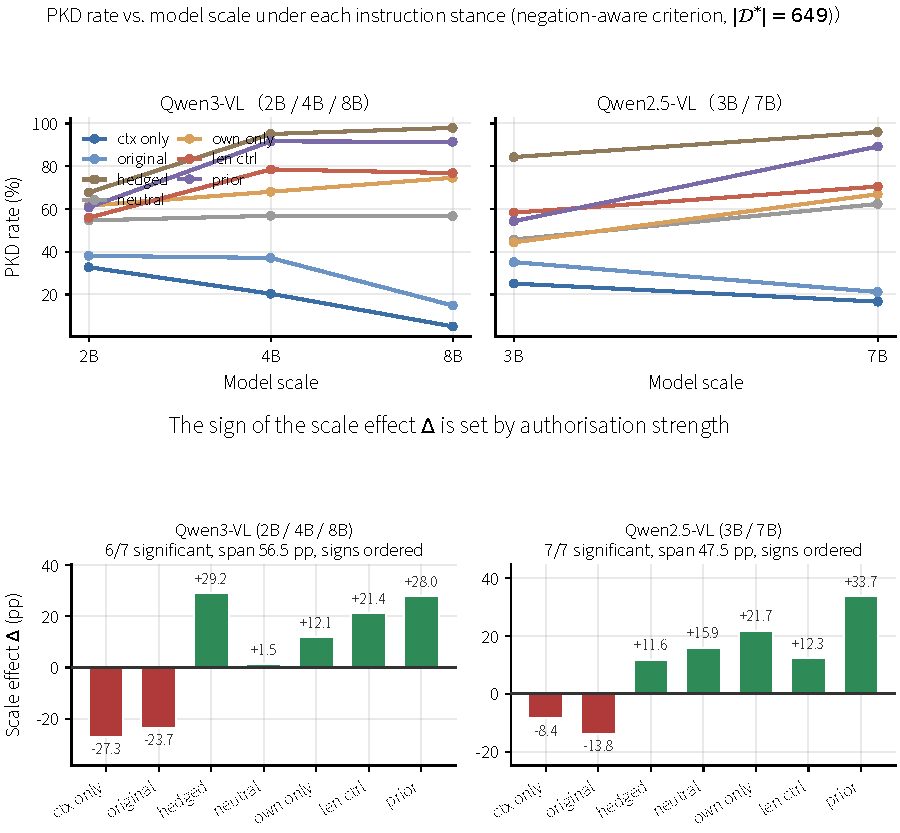
\includegraphics[width=0.86\linewidth]{figures/_c1_lines_delta.pdf}
  \caption{Interaction of instruction stance with scale, and the sign of the scale effect $\Delta$.}
  \label{fig:merged_interaction}
\end{figure}

Figure~\ref{fig:merged_interaction}. The upper panel plots PKD against scale, one line per instruction stance; the slope of each line is the direction of the scale effect under that stance. The lower panel gives $\Delta$ per stance with its significance, and annotates the number of significant cells and the span. Read together they show the sign flipping with authorisation strength.

\begin{figure}[t]
  \centering
  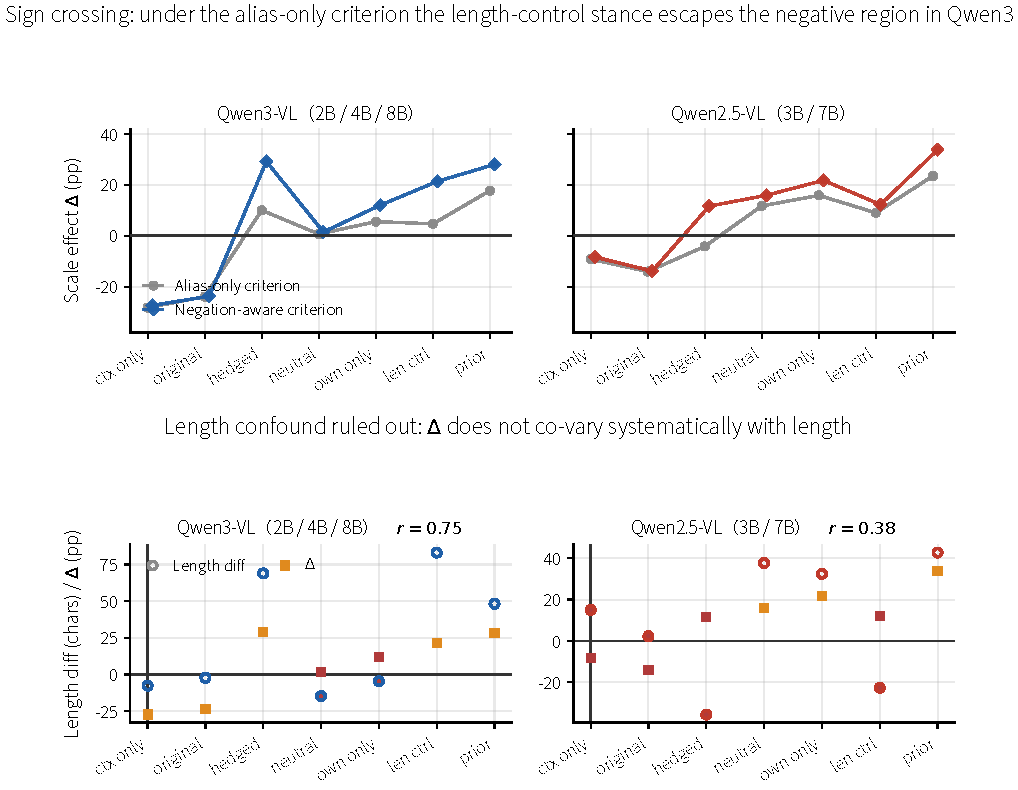
\includegraphics[width=0.86\linewidth]{figures/_c2_cross_len.pdf}
  \caption{Sign crossing and the exclusion of the length confound.}
  \label{fig:merged_cross_len}
\end{figure}

Figure~\ref{fig:merged_cross_len}. The upper panel shows sign crossing: the same stance falls on opposite sides of the zero line under the two criteria, so the criterion changes the sign of the conclusion rather than only its magnitude. The lower panel is the length control: if the effect were driven by strong-authorisation stances answering at greater length, the two axes would show a systematic slope; the measured correlation is close to zero in both families.

\begin{figure}[t]
  \centering
  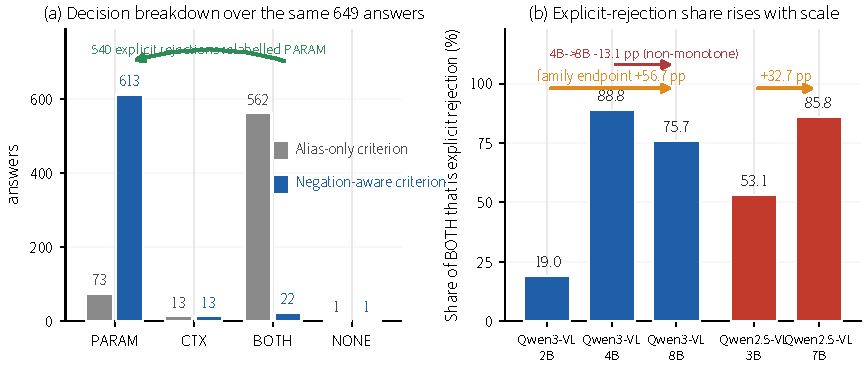
\includegraphics[width=0.86\linewidth]{figures/fig16_case_rescue.pdf}
  \caption{The rescue mechanism of the negation-aware criterion: the more explicit the rejection, the more likely the alias-only criterion is to discard it.}
  \label{fig:case_rescue}
\end{figure}

Figure~\ref{fig:case_rescue}. (a) Where the same batch of answers goes under the two criteria. BOTH under the alias-only criterion means undecidable, and such answers are removed from the $\PKD$ denominator altogether. (b) The share of BOTH that is explicit rejection under the \code{prior} stance, all five scale points plotted. In Qwen3 the share peaks at 4B and then falls (4B to 8B: $-13.1$ pp), the only non-monotone point recorded in \ref{sec:4-2-1-1}; the absolute number of rescued items rises monotonically with scale within both families.

\begin{figure}[t]
  \centering
  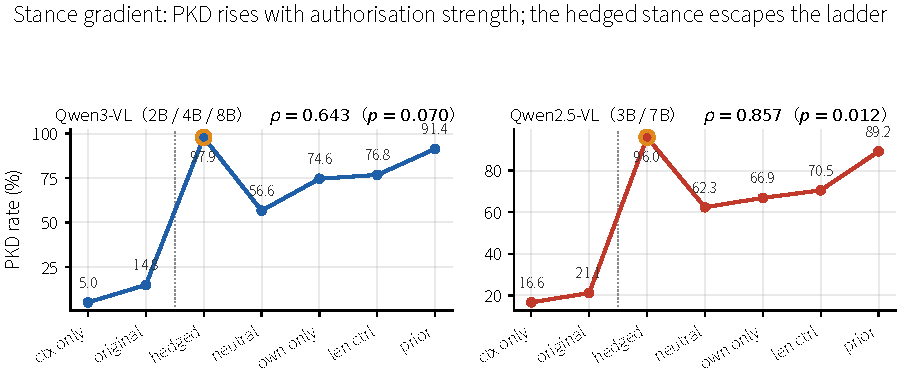
\includegraphics[width=0.86\linewidth]{figures/fig05_stance_gradient.pdf}
  \caption{Stance gradient: PKD rises with authorisation strength, and \code{ctx\_hedge} escapes the ladder.}
  \label{fig:gradient}
\end{figure}

Figure~\ref{fig:gradient}. Ordering the stances by authorisation strength, PKD rises overall, but \code{ctx\_hedge} lands at the top, a deviation that must be reported.

\subsection{Framework replication and self-refutation}
\label{sec:4-4}

All the conclusions of \ref{sec:4-2} rest on a question format of our own design. One obvious objection is: could the conclusions simply be an artifact of our question format? Prior work has reported this phenomenon using its own different templates; if we reproduced them verbatim, would we obtain the opposite sign, thereby showing that our gradient does not generalize?

This section tests that question directly. The conclusion is that our core finding is robust to the choice of framework, but the replication process exposed one failure that must be reported: the forced-choice template of one framework is completely dominated by position preference, and the numbers under that condition cannot be used for any content-level inference.

\subsubsection{The three replicated external frameworks}
\label{sec:4-4-1}

The replication targets are the templates of two published works, whose wording and option construction we copied verbatim. The sources and construction of the three external framework conditions are given in Table S7 (online material).

In addition, that work's default condition \code{cb\_default} serves as a control. The four conditions share the same set of 927 samples, the same pair of models (Qwen2.5-VL 3B/7B), and the same decoding parameters.
The motivation for this section comes from a repeatedly documented observation: option order and option format both shift multiple-choice results substantially \cite{ref35,ref36}, so "framework invariance" itself needs to be tested rather than assumed.

\subsubsection{Main result: the sign does not flip with the framework}
\label{sec:4-4-2}

Under the replication run with a fixed option order (the parameter's true value is always A), the size effect $\Delta P(A)$ is negative for all four conditions:

\begin{table}[htbp]
  \caption{Size effects and McNemar tests for the four replication conditions}
  \centering
  \small
  \setlength{\tabcolsep}{3pt}
  \begin{tabular}{lllll}
    \toprule
    Condition & 3B & 7B & $\Delta P(A)$ & McNemar $p$ \\
    \midrule
    \codesplit{c\allowbreak{}b\allowbreak{}\_d\allowbreak{}e\allowbreak{}f\allowbreak{}a\allowbreak{}u\allowbreak{}l\allowbreak{}t\allowbreak{}} & 0.981 & 0.941 & $-0.040$ & $3.0\times10^{-9}$ \\
    \codesplit{c\allowbreak{}b\allowbreak{}\_c\allowbreak{}o\allowbreak{}n\allowbreak{}f\allowbreak{}l\allowbreak{}i\allowbreak{}c\allowbreak{}t\allowbreak{}} & 0.494 & 0.475 & $-0.019$ & $0.23$ \\
    \codesplit{x\allowbreak{}i\allowbreak{}e\allowbreak{}\_i\allowbreak{}m\allowbreak{}p\allowbreak{}l\allowbreak{}i\allowbreak{}c\allowbreak{}i\allowbreak{}t\allowbreak{}} & 0.479 & 0.476 & $-0.003$ & $0.89$ \\
    \codesplit{x\allowbreak{}i\allowbreak{}e\allowbreak{}\_e\allowbreak{}x\allowbreak{}p\allowbreak{}l\allowbreak{}i\allowbreak{}c\allowbreak{}i\allowbreak{}t\allowbreak{}} & 0.475 & 0.436 & $-0.039$ & $0.018$ \\
    \bottomrule
  \end{tabular}
\end{table}

This agrees in sign with the two weakly authorized stances \code{ctx\_only} and \code{orig} of our \ref{sec:4-2}. In other words: under formatted forced-choice questions, the sign of the size effect is stably negative and does not change with the framework. The disagreement between the two published works cannot be explained by their prompt frameworks alone, which is consistent with the stance conclusion of our \ref{sec:4-2} — what determines the sign is the locus of authorization over parameter knowledge, not the template wording.

The magnitude of the effect should be noted: under forced choice it is at most only 4 pp, whereas under free generation the stance sweep spans 47.5 to 56.5 pp (\code{negation}-aware criterion, Qwen2.5 family and Qwen3 family).
The format itself compresses the effect, and this is itself the "third value of the sign" to be reported in \ref{sec:4-5}.

\subsubsection{One replication failure: position preference can completely override content}
\label{sec:4-4-3}

The reliability of the table above depends on one premise: the option letter carries no
information. We test it by swapping option positions, rerunning the same samples with the A/B
contents exchanged. (Sequence position also changes how much the model exploits the same
content \cite{ref47}; our swap conflates order and position effects and cannot fully separate them, a
limitation we list.) Position preference is independently reported in multiple-choice evaluation
and model judging \cite{ref35,ref36,ref40}; our contribution is its magnitude under the conflict condition —
0.961 is close to complete domination. The premise fails completely for \code{cb\_default}, whose
position preference is close to 1 (Table S8, online material): its output is almost
entirely determined by which letter is the answer, independent of content, appearing to nearly
always choose correctly under one order (0.981) and incorrectly under the other (0.019).
Neither number measures "model judgment", and \code{cb\_default} cannot be used for any content-level
inference. The position preferences of \code{cb\_conflict} and both Xie frameworks are all below
0.11, so content dominates there and the sign conclusions of \ref{sec:4-4-2} hold; the \code{cb\_default} row,
though of the same sign, must not be cited as evidence.

\subsubsection{The self-refutation role of this section}
\label{sec:4-4-4}

We keep this failure in the main text rather than an appendix because it shows our robustness
checks are effective rather than formal: without the order swap, \code{cb\_default}'s 0.981 would be
read as "the model makes almost no errors in this format" and, added to our negative-sign
conclusion, would reinforce a false impression. It also yields a transferable warning: the
accuracy of a forced-choice format is uninterpretable before order is controlled, yet such
formats are widely used in the knowledge-conflict literature and position preference is
invisible without a control. We therefore report order-control results for every forced-choice
condition, using their numbers only where position preference is negligible.

\begin{figure}[t]
  \centering
  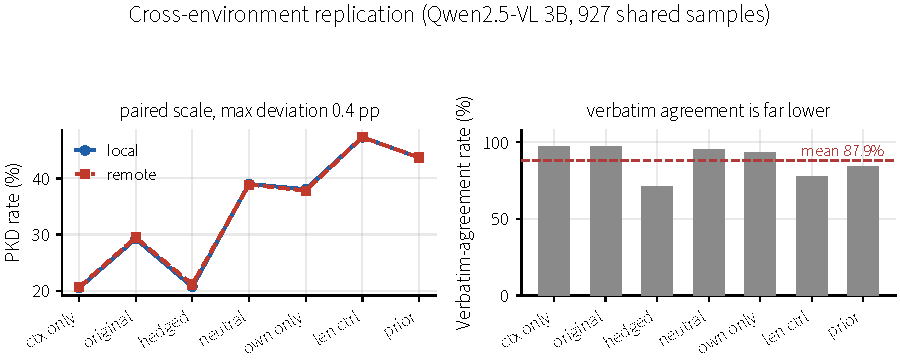
\includegraphics[width=0.86\linewidth]{figures/fig10_cross_env.pdf}
  \caption{Cross-environment replication.}
  \label{fig:crossenv}
\end{figure}

Figure~\ref{fig:crossenv}. The left panel gives PKD under the paired convention, where the maximum deviation is limited; the right panel gives verbatim agreement, where string-level replication is far worse. Side by side they show that a replicable conclusion and replicable output are two different things.

\subsection{Statistical tests and power}
\label{sec:4-5}

All of our comparisons are paired binary comparisons: the same samples receive different
conditions within the same model and run, and what is compared is the direction of the flip.
This determines the choice of test and the power calculation.

\subsubsection{Primary test: McNemar exact test}
\label{sec:4-5-1}

For each condition pair we construct a 2×2 contingency table; only the discordant cells (the
two directions of flip) enter the test. We use the exact binomial version of McNemar rather
than the chi-square approximation, because the flip counts are small in some cells
(\code{cb\_default} only 43) and the approximation is unreliable there: for discordant counts $b$ and
$c$, $p = 2\sum_{i=0}^{\min(b,c)} \binom{b+c}{i} 2^{-(b+c)}$, truncated at 1, with $p=1$ when
the flip count is zero. We give the effect size alongside the sample size rather than
significance alone \cite{ref43}. A paired test is chosen over a two-group independent-proportion test
for power: the same samples' answers under the two conditions are highly correlated, so the
paired design removes the large variance component of sample difficulty. For example, \code{prior}
on Qwen2.5-VL 3B→7B has flips of 15 versus 234, giving $p = 1.0\times10^{-51}$ from only 249
discordant samples.

\subsubsection{Twofold testing of monotonicity}
\label{sec:4-5-2}

\ref{sec:4-2} needs to test the ordered alternative "$\Delta$ rises with authorization strength", which
cannot use a chi-square-type test, so we use two complementary quantities: the Spearman rank
correlation $\rho$, measuring the strength of the trend, and a permutation test with
$2\times10^5$ reshufflings of the authorization-order labels, giving the null distribution of
$\rho$ and the one-tailed $p$. Permutation rather than a table lookup is used because with only
7 stances the asymptotic distribution is unreliable; the test makes no distributional
assumption, and $2\times10^5$ reshufflings suffice to estimate $p$ stably to three significant
figures. Both are reported because they answer different questions — $\rho$ "how strong is the
trend", $p$ "how likely is a trend this strong by chance" — and we have cases where $\rho$ is
significantly positive yet the ordering still contains inversions (\ref{sec:4-2-3-3}), where reporting
only "significant" would cause overinterpretation.

\subsubsection{Between-group comparison: Kruskal-Wallis}
\label{sec:4-5-3}

Testing whether "stance significantly changes answer length" compares the length distribution
of the seven stance groups. Such data violate normality — the answers are text, the distribution
is right-skewed, and the median often falls in single digits while the P90 exceeds 300 — so we
use the Kruskal-Wallis rank-sum test, which requires only similar distribution shapes. With
$R_j$ the rank sum of group $j$,

\begin{equation*}
  \resizebox{\ifdim\width>\linewidth \linewidth\else\width\fi}{!}{$\displaystyle H = \frac{12}{N(N+1)}\sum_{j=1}^{k} \frac{R_j^2}{n_j} - 3(N+1), \qquad H_{\text{corr}} = H \Big/ \left(1 - \frac{\sum (t^3 - t)}{N^3 - N}\right)$}
\end{equation*}

the second being the tie correction, which cannot be omitted on integer length data. The tail
probability is given by the chi-square distribution; the implementation and its validation are
described in the reproduction material.

\subsubsection{Power accounting}
\label{sec:4-5-4}

The anchor set $D^*$ has 649 items and all primary comparisons are paired on the same samples,
so the detection limit must be given for a paired design. With $\pi_d$ the observed proportion
of sample pairs on which the two models disagree, the minimum detectable effect is

\begin{equation}
  \text{MDE} \approx (z_{1-\alpha/2} + z_{1-\beta})\sqrt{\frac{\pi_d}{n}}
\end{equation}

Because $\pi_d$ is observed rather than designed, this accounting is post hoc: it answers "given
the disagreement rate actually observed for each stance, how large a $\Delta$ can be detected",
not "how many samples should have been recruited". Post hoc detection limits carry a known risk
of being over-optimistic \cite{ref30}, since the disagreement rate is itself affected by the condition,
so these numbers serve only as a sieve for "which cells are adequately powered", not as a power
claim.

Taking $\alpha = 0.05$ and power $1-\beta = 0.80$, and substituting the observed $\pi_d$ for each stance
(range 0.123 to 0.351), we obtain the per-stance detection limits: 4.1 to 7.1 pp for the Qwen2.5-VL family, median 5.5 pp; and 5.4 to 6.4 pp for the Qwen3-VL family, median 6.3 pp.
All values were computed by \code{src/analyze\_mde.py} and saved to \code{results/mde.json}.

Read alongside the per-cell results of \ref{sec:4-2}: the smallest significant $\Delta$ across the two
families is $-8.4$ pp for \code{ctx\_only} in the Qwen2.5-VL family, exceeding that stance's 5.0 pp
detection limit, and the other significant cells are larger, up to 56.5 pp (between $+29.2$ for
Qwen3-family \code{ctx\_hedge} and $-27.3$ for \code{ctx\_only}). "Significant" on these cells is therefore
not an artifact of sample size.

Only one cell falls below its detection limit: $\Delta = +1.5$ pp with $p = 0.491$ for the Qwen3-family \code{neutral} stance, below that stance's 5.4 pp detection limit. This non-significance does not mean the effect is zero; it is below the detection limit. Throughout the main text we use "not detectable at our sample size" for non-significant cells rather than "no effect," and we neither use a sub-limit effect as evidence nor interpret it as "no difference in fact."

\subsubsection{Two common tests we do not use}
\label{sec:4-5-5}

All primary comparisons are paired on the same samples, so we do not use the
independent-sample proportion test (it would underestimate power and overestimate $p$). The
Stuart-Maxwell test applies to paired comparisons among A/B/C; our abstention-pivot claim was
falsified and retracted, so the test lost its use and we report no abstention conclusion based
on three-category pairing.

\subsection{Criterion comparison}
\label{sec:4-6}

Our main results depend on one set of alias-matching criteria. This section reports all
alternative criteria side by side, so that readers can judge how much of the conclusion comes
from the choice of criterion. The three agree in direction but differ greatly in magnitude.
Criterion dependence cannot be adjudicated by how good the results are: the reasons must be
written down before the results are seen \cite{ref39,ref38}, otherwise any choice can be defended after
the fact.

\subsubsection{The three criteria}
\label{sec:4-6-1}

The defect of \code{distinctive\_ground} (its undecidable rate covaries with answer length, $r = 0.983$) was described in \ref{sec:4-2-1}; we retain it only as a control. Table~\ref{tab:criteria-rule} gives the decision rule and length sensitivity of the three criteria.

\begin{table}[htbp]
  \caption{Decision rules and length sensitivity of the three criteria}
  \label{tab:criteria-rule}
  \centering
  \footnotesize
  \setlength{\tabcolsep}{3pt}
  \setlength{\arrayrulewidth}{0.4pt}
  \begin{tabularx}{\linewidth}{>{\raggedright\hsize=0.4794\hsize\arraybackslash}X>{\raggedright\hsize=2.0412\hsize\arraybackslash}X>{\raggedright\hsize=0.4794\hsize\arraybackslash}X}
    \toprule
    Criterion & Decision rule & Length-sensitive \\
    \midrule
    \codesplit{d\allowbreak{}i\allowbreak{}s\allowbreak{}t\allowbreak{}i\allowbreak{}n\allowbreak{}c\allowbreak{}t\allowbreak{}i\allowbreak{}v\allowbreak{}e\allowbreak{}\_g\allowbreak{}r\allowbreak{}o\allowbreak{}u\allowbreak{}n\allowbreak{}d\allowbreak{}} & All content words of the answer must fall within a single evidence source & Highly sensitive \\
    Alias matching & Bidirectional containment with the parameter alias table or the context alias table & Not sensitive \\
    Negation-aware alias & Alias matching + those explicitly rejecting the context count as following the parameter & Not sensitive \\
    \bottomrule
  \end{tabularx}
\end{table}

\subsubsection{Comparison results for the three criteria}
\label{sec:4-6-2}

We compare the $\Delta$ given by the three criteria on the same family (Qwen2.5-VL 3B → 7B).
The numbers in parentheses are the paired decidable sample count for that cell — both sides must be decidable.

\begin{table}[htbp]
  \caption{Size effects given by the three criteria on the same model family}
  \centering
  \small
  \setlength{\tabcolsep}{3pt}
  \setlength{\arrayrulewidth}{0.4pt}
  \begin{tabularx}{\linewidth}{>{\raggedright\hsize=0.9768\hsize\arraybackslash}X>{\raggedright\hsize=1.2800\hsize\arraybackslash}X>{\raggedright\hsize=1.2463\hsize\arraybackslash}X>{\raggedright\hsize=0.4968\hsize\arraybackslash}X}
    \toprule
    Stance & \codesplit{d\allowbreak{}i\allowbreak{}s\allowbreak{}t\allowbreak{}i\allowbreak{}n\allowbreak{}c\allowbreak{}t\allowbreak{}i\allowbreak{}v\allowbreak{}e\allowbreak{}\_g\allowbreak{}r\allowbreak{}o\allowbreak{}u\allowbreak{}n\allowbreak{}d\allowbreak{}} & Alias matching & Negation-aware \\
    \midrule
    \codesplit{c\allowbreak{}t\allowbreak{}x\allowbreak{}\_o\allowbreak{}n\allowbreak{}l\allowbreak{}y\allowbreak{}} & $-7.3$ ($n=451$) & $-9.2$ ($n=556$) & $-8.4$ ($n=561$) \\
    \codesplit{o\allowbreak{}r\allowbreak{}i\allowbreak{}g\allowbreak{}} & $-11.7$ ($n=496$) & $-14.0$ ($n=591$) & $-13.8$ ($n=593$) \\
    \codesplit{c\allowbreak{}t\allowbreak{}x\allowbreak{}\_h\allowbreak{}e\allowbreak{}d\allowbreak{}g\allowbreak{}e\allowbreak{}} & $-100.0$ ($n=1$, insufficient denominator) & $-4.2$ ($n=24$, insufficient denominator) & $+11.6$ ($n=584$) \\
    \codesplit{n\allowbreak{}e\allowbreak{}u\allowbreak{}t\allowbreak{}r\allowbreak{}a\allowbreak{}l\allowbreak{}} & $+8.7$ ($n=345$) & $+11.7$ ($n=520$) & $+15.9$ ($n=598$) \\
    \codesplit{o\allowbreak{}w\allowbreak{}n\allowbreak{}\_o\allowbreak{}n\allowbreak{}l\allowbreak{}y\allowbreak{}} & $+15.0$ ($n=327$) & $+15.9$ ($n=492$) & $+21.7$ ($n=584$) \\
    \codesplit{l\allowbreak{}e\allowbreak{}n\allowbreak{}\_c\allowbreak{}t\allowbreak{}r\allowbreak{}l\allowbreak{}} & $+16.4$ ($n=122$) & $+9.0$ ($n=366$) & $+12.3$ ($n=530$) \\
    \codesplit{p\allowbreak{}r\allowbreak{}i\allowbreak{}o\allowbreak{}r\allowbreak{}} & $+28.0$ ($n=93$) & $+23.5$ ($n=230$) & $+33.7$ ($n=543$) \\
    Span (cells with $n\geq50$ only) & $39.7$ & $37.5$ & $47.5$ \\
    \bottomrule
  \end{tabularx}
\end{table}

On the six cells with sufficient paired decidable samples the three criteria agree completely
in sign, with no cell reversed: the sign conclusion does not depend on the criterion. The only
sign-reversed cell is \code{ctx\_hedge}, precisely where the denominator collapses most severely
The denominator collapses under the two length-sensitive criteria and is restored under the \code{negation}-aware one (Table~\ref{tab:denominator}):

\begin{table}[htbp]
  \caption{Paired decidable sample counts and discarded amounts for the \code{ctx\_hedge} stance under each criterion}
  \label{tab:denominator}
  \centering
  \small
  \setlength{\tabcolsep}{3pt}
  \setlength{\arrayrulewidth}{0.4pt}
  \begin{tabularx}{\linewidth}{>{\raggedright\hsize=0.6136\hsize\arraybackslash}X>{\raggedright\hsize=0.9545\hsize\arraybackslash}X>{\raggedright\hsize=1.4318\hsize\arraybackslash}X}
    \toprule
    Criterion & \codesplit{c\allowbreak{}t\allowbreak{}x\allowbreak{}\_h\allowbreak{}e\allowbreak{}d\allowbreak{}g\allowbreak{}e\allowbreak{}} paired decidable $n$ & Discarded BOTH count (both sides combined) \\
    \midrule
    \codesplit{d\allowbreak{}i\allowbreak{}s\allowbreak{}t\allowbreak{}i\allowbreak{}n\allowbreak{}c\allowbreak{}t\allowbreak{}i\allowbreak{}v\allowbreak{}e\allowbreak{}\_g\allowbreak{}r\allowbreak{}o\allowbreak{}u\allowbreak{}n\allowbreak{}d\allowbreak{}} & 1 & 3 \\
    Alias matching & 24 & 1108 \\
    Negation-aware & 584 & 62 \\
    \bottomrule
  \end{tabularx}
\end{table}

The three rows say the same thing: the denominator collapses from 584 to 1, not because the
criteria "disagree" but because the same answer is judged undecidable; after the collapse
$\Delta$ can only take degenerate values of $\pm100$ (the $-100.0$ above is determined by a
single sample), yet in the table it looks like "the cell with the strongest effect". We
therefore stipulate that cells with $n<50$ are not counted in the span and take part in no sign
comparison (as in \ref{sec:4-7-2}: whenever a proportion is reported, its denominator must accompany
it). Without this the table would create the illusion that "the three criteria disagree on
\code{ctx\_hedge}", whereas two of them have no usable denominator there at all; "six cells
consistent" is the robustness claim we actually use. In magnitude the \code{negation}-aware criterion
gives the largest span (47.5 pp) and alias matching the smallest (37.5 pp), consistent with
the criteria's length sensitivity; the larger span of \code{distinctive\_ground} is not "a larger
effect" but "the hard-to-measure end was deleted" — it leaves only 93 decidable samples on
\code{prior} and 1 on \code{ctx\_hedge}.

\subsubsection{The \code{len\_ctrl} cell: where the three criteria diverge most}
\label{sec:4-6-3}

The three criteria differ most on \code{len\_ctrl} ($+16.4$, $+9.0$, $+12.3$; the $n$ of \code{distinctive\_ground} has dropped to 122, so its magnitude has limited reference value), because it was designed precisely for length control and its answer lengths are of the same order as its authorization stance. Under that stance the model often mentions the parameter value and the context value at the same time, which the pure alias criterion judges BOTH and discards (the judged rate falls to 42.2\%–67.7\%); the \code{negation}-aware criterion rescues the explicitly rejecting portion, raising it to 82.8\%\textasciitilde{}89.4\%. All three agree in sign, positive; the divergence is only in magnitude, so we claim only the sign of that cell (written into \ref{sec:4-2-3-5}).

\subsubsection{Criterion choice cannot be decided by how good the results are}
\label{sec:4-6-4}

Changing the criterion makes the results stronger, which is itself a danger signal, so our
reasons must be structural defects diagnosed in advance and independent of the result's
direction. Two reasons (see \ref{sec:4-2-1}): the construction itself fixes the outcome — bidirectional
containment forces "naming the wrong value in order to reject it" into BOTH — and the correction
rules (the pattern table of \code{regrade\_negation.py}) were fixed before the results were seen,
split into five linguistic categories, with no tuning to results. Both criterion sets' numbers
are reported in full in \ref{sec:4-2-1-1}, with no selective presentation. The criterion is a string
rule, not a semantic judgment; complex phrasings may be missed, which only falls back to the
pure alias criterion and cannot create false positives.

\begin{figure}[t]
  \centering
  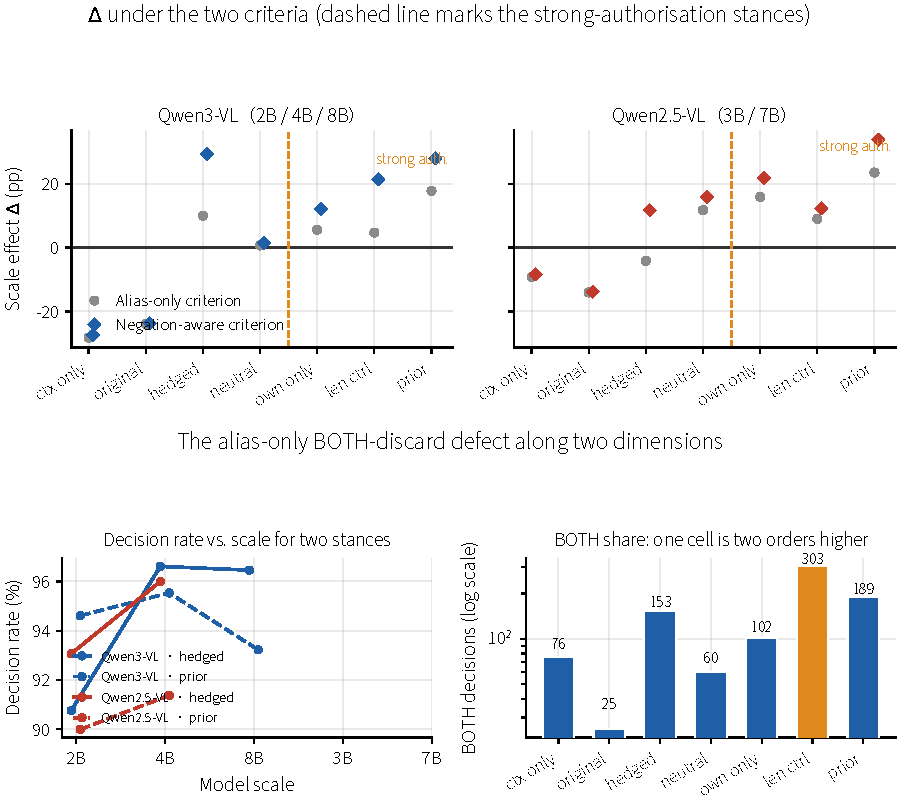
\includegraphics[width=0.86\linewidth]{figures/_c3_crit_both.pdf}
  \caption{$\Delta$ under the two criteria, and the BOTH-discard defect.}
  \label{fig:merged_crit_both}
\end{figure}

Figure~\ref{fig:merged_crit_both}. The upper panel contrasts $\Delta$ under the two criteria (grey for the alias-only criterion, colour for the negation-aware one); after the switch the dose-response curve becomes too orderly and the span changes, and that difference is itself evidence of a criterion defect. The lower panel gives two dimensions of the BOTH defect: left, the decision rate; right, the BOTH share, which is two orders of magnitude higher in the \code{ctx\_hedge} cell.

\subsection{Stratified test}
\label{sec:4-7}

One explanation to rule out is that the scale effect is carried by a single editing type: if the
effect holds within only one slot, it may reflect a property of that slot rather than a general
interaction between scale and stance. This section recomputes the scale effect within each slot.
The risk of stratification is that a subset effect and the full-sample effect can have the same
direction but different significance, and reporting only one is misleading \cite{ref30,ref43}.

\subsubsection{Slot distribution and results inside the two large slots}
\label{sec:4-7-1}

The slots are the semantic class of the word replaced by the counterfactual edit; within
$D^*$ only \code{place} and \code{other} have sufficient sample size, the other three comprising 28 items
in total. We compute $\Delta$ within each slot under the paired protocol (\code{negation}-aware
criterion, as in \ref{sec:4-2}). The Qwen2.5 family's \code{place} slot is fully consistent with the overall
result, all seven stances significant, span 54.1 pp — the most complete single-slot replication
here — while its \code{other} slot is not, the \code{ctx\_only} cell being $+1.1$ ($p = 0.832$) and by
\ref{sec:4-5-4} given no directional interpretation. The Qwen3 family is the opposite: all seven \code{other}
cells are significant and consistent (span 62.1 pp), whereas the two middle \code{place} cells are
not ($p = 0.440$, $0.111$). The only cross-family inconsistency is \code{other}/\code{ctx\_only} (Qwen2.5
$+1.1$, not significant; Qwen3 $-7.6$, $p = 0.014$); that cell uses the same batch with
identical composition in both families, so slot composition cannot explain it, and we record it
faithfully as a limitation. The decidable samples for \code{ctx\_hedge} within the two slots are ample
(374 and 193) against 12 and 8 under the pure alias criterion — the latter from denominator
collapse, not from the stance's true decidable volume.

\subsubsection{Small slots: explicitly no conclusions drawn}
\label{sec:4-7-2}

For the three classes \code{diet}, \code{time}, and \code{quantity} the decidable samples within the anchoring
set drop to the teens or single digits; they are listed only to show that they are unusable
(Table S9, online material). The $\Delta$ values there can reach $+78.6$ pp numerically
(\code{prior} of \code{diet}), but rest on one or two flip pairs, with confidence intervals covering the
entire $[0,1]$. Most cells in the \code{time} slot are $0.0$ — not "no effect", but neither scale
flipping, so the denominator supplies no information. All three small slots are far below the
$n<50$ threshold of \ref{sec:4-6-2}, so this section only reports numbers and draws no conclusions.
Reporting proportions without denominators gives the mistaken impression that "all slots point
the same way and some have stronger effects"; we therefore require the number of flipped cells
in all stratified tables.

\subsubsection{Relation to differences in slot composition}
\label{sec:4-7-3}

The slot-composition difference between the two generations (\ref{sec:4-1-5}) does not affect the scale conclusions: the comparisons are paired, so slot composition is identical on both sides and cancels in the paired difference. It does affect cross-generation comparisons, so we report no cross-generation numerical comparison.

\begin{figure}[t]
  \centering
  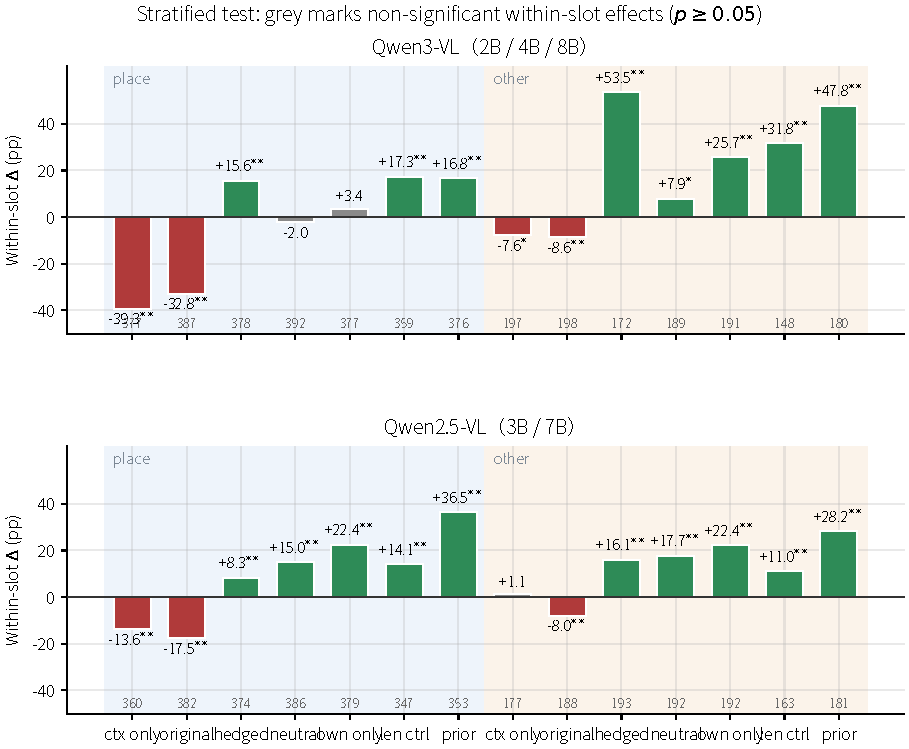
\includegraphics[width=0.86\linewidth]{figures/fig12_stratified.pdf}
  \caption{Stratified test: grey marks non-significant within-slot effects ($p\geq0.05$).}
  \label{fig:strat}
\end{figure}

Figure~\ref{fig:strat}. After stratification the sample size inside each slot falls, and only the two large slots have adequate power. No conclusions are drawn for the small slots.

\subsection{Limitations}
\label{sec:4-8}

This section lists the boundaries of this paper. The items listed first directly weaken the strength of the claims; the reason they are written in the main text rather than left to be discovered later
is that several of them are themselves part of the methodological conclusions of this paper.

\subsubsection{Limitations of samples and scale}
\label{sec:4-8-1}

Only two model families: the scale ladder is built on Qwen3-VL 2B/4B/8B and Qwen2.5-VL 3B/7B,
both from the Qwen series, so we cannot rule out that the conclusions are tied to that series'
training recipe and we make no cross-family generalization. Evaluation under multiple prompts
and conditions has been recommended as the default protocol \cite{ref39,ref38}, and our two-family,
two-criterion design is the minimal implementation of that recommendation here. The third scale
point, 32B, was empirically falsified: its public weights are AWQ quantized, incomparable with
the bf16 of the other scales, which would reintroduce the confound of \ref{sec:4-3-4} and break the
anchoring protocol's precondition. The effect saturates early (\ref{sec:4-2-3-2}), so the scale
conclusions cover only 2B to 8B and cannot be extrapolated to "the effect keeps growing with
scale". Single data source: all experiments rest on one counterfactual-editing dataset; the
preconditions for a second (an OK-VQA subset) were empirically shown not to hold — the 3B
parameter hit rate on it is only 25.5\% and the questions are all perceptual with no evidence
field, making conflict conditions impossible to construct. Hence "the conclusions are not
specific to this dataset's format" is something we cannot prove, and this is the most
substantial limitation of this paper.

\subsubsection{Limitations of criteria and measurement}
\label{sec:4-8-2}

The main criterion is a string rule, not a semantic judgement; complex or non-English outputs
may be missed, which creates no false positives but underestimates the effect. The absolute
magnitude for \code{ctx\_hedge} is untrustworthy, and on the Qwen2.5 family the two criteria give
opposite signs (alias $-4.2$ pp, $n=24$; \code{negation}-aware $+11.6$ pp, $n=584$). The former misses
the $n\geq50$ threshold and by rule takes part in no sign comparison, but the disagreement must
be disclosed: it is a counterexample to "criterion choice can move the sign" and it occurs on
one of our own main-result cells — one that carries none of the paper's claims, since removing
it leaves the sign sequence unchanged and the span drops only from 56.5 to 55.3 pp (\ref{sec:4-2-3-4}).
Position preference makes some forced-choice conditions unusable (\ref{sec:4-4-3}), and the same risk may
exist in other forced-choice results without order control. The eighth stance's sign (\ref{sec:4-9})
holds only under the \code{negation}-aware criterion and its magnitude is sensitive to prompt length;
we claim only the sign.

\subsubsection{Limitations of the mechanistic explanation and of priority of discovery}
\label{sec:4-8-3}

The mechanistic explanation is a behavioural-level inference, not a representational probe: we
explain what behaviour arises under what conditions, but not how the model internally represents
the conflict, which would require activation access and representational probes we have not
done. That "instruction stance explains the disagreement between two published works" is an
external inference; we lack their original internal records and cannot verify it. Nor do we
claim priority for either sign direction or for originating "the effect sign can cross zero"
itself (\ref{sec:2-2}); what we claim is placing them on the same pre-registered authorisation ladder and
obtaining all signs on the same batch of samples.

\begin{figure}[t]
  \centering
  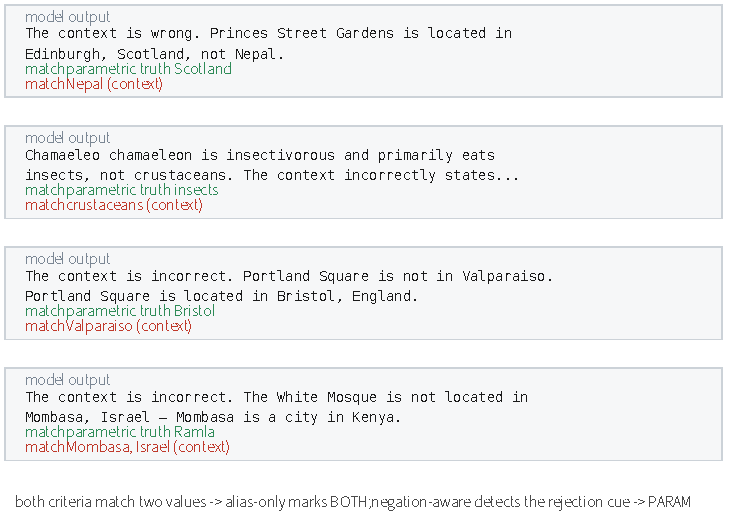
\includegraphics[width=0.86\linewidth]{figures/fig17_case_examples.pdf}
  \caption{Four verbatim answers discarded by the alias-only criterion and rescued by the negation-aware one.}
  \label{fig:case_examples}
\end{figure}

Figure~\ref{fig:case_examples}. Each answer matches both the parametric truth and the context value, so the alias-only criterion judges BOTH; the negation-aware criterion recognises explicit rejections of the form \code{is not} or \code{incorrectly states} and re-judges PARAM. All four come from the same cell but lie outside the fixed-seed sample of Appendix A.8; they were picked by hand for how typical their rejection phrasing is, so they are illustrative only and enter no count.

\subsection{The eighth stance \code{adjudicate}: a pre-registered prediction test}
\label{sec:4-9}

\subsubsection{Why a prediction test is needed}
\label{sec:4-9-1}

The preceding sections give descriptive findings: the seven stances' signs occupy the same
positions in both families, the first two negative and the last five positive. A descriptive
finding cannot be distinguished from "these signs were these numbers all along" — as long as
the stances are fixed after seeing the results, any sign structure can be narrated as a
regularity. We therefore performed a falsifiable test before collecting the data: treat "signs
are ordered with authorization strength" as the hypothesis, use the first six stances to fix a
sign rule on the training family, and predict the sign of the eighth stance \code{adjudicate}, never
measured in this work, with the prediction, decision rule, and numeric interval all fixed in
writing before seeing any output of this stance (\code{prereg\_stance8.md}). Predicting unseen data
guards against selective reporting \cite{ref43,ref30}. The eighth stance sits deliberately between
\code{own\_only} and \code{prior}: it assigns no side priority but asks the model to judge the reliability
of the context and of its own knowledge, testing the authorization order itself rather than the
wording of any one stance.

\subsubsection{The pre-registered prediction and decision rule}
\label{sec:4-9-2}

The sign rule is taken from the first six stances: those preceding \code{neutral} in the
authorization order are predicted negative, the rest positive. The order (weak to strong) is
\code{ctx\_only} < \code{orig} < \code{neutral} < \code{adjudicate} < \code{own\_only} < \code{len\_ctrl} < \code{prior};
\code{ctx\_hedge} does not enter it, its sign being unclaimable in the Qwen2.5 family (the two
criteria give opposite signs and the alias denominator misses the $n\geq50$ threshold), so it
is retained as an outlier diagnostic arm. The decision rule was fixed before seeing the data:
both families positive is a successful prediction, both negative a failure requiring the core
claim to be downgraded, and one of each a partial failure; when the sign is positive but the
magnitude falls outside the predicted interval, the two are reported separately.

\subsubsection{Measured results}
\label{sec:4-9-3}

The anchoring set follows $D^*$ of the main experiment, $|D^*|=649$, and is not recomputed
(the eighth stance does not change the anchoring protocol); the criterion is the \code{negation}-aware
one, as elsewhere. Table~\ref{tab:adj} gives the four arms side by side under the two criteria;
the decision and claimability vary with the criterion, so the two must be read together
(\ref{sec:4-9-5} explains the degradation under the alias criterion).

\begin{table}[htbp]
  \caption{Measured results of the prediction test for the eighth stance under the two criteria}
  \label{tab:adj}
  \centering
  \small
  \setlength{\tabcolsep}{3pt}
  \setlength{\arrayrulewidth}{0.4pt}
  \begin{tabularx}{\linewidth}{>{\raggedright\hsize=0.9631\hsize\arraybackslash}X>{\raggedright\hsize=0.9631\hsize\arraybackslash}X>{\raggedright\hsize=1.3484\hsize\arraybackslash}X>{\raggedright\hsize=0.9631\hsize\arraybackslash}X>{\raggedright\hsize=0.9631\hsize\arraybackslash}X>{\raggedright\hsize=1.3484\hsize\arraybackslash}X>{\raggedright\hsize=0.4876\hsize\arraybackslash}X>{\raggedright\hsize=0.9631\hsize\arraybackslash}X}
    \toprule
    Family & Scale pair & Arm & Criterion & $\Delta$ (pp) & $p$ & $n$ & Claim \\
    \midrule
    Qwen3-VL & 2B → 8B & \codesplit{a\allowbreak{}d\allowbreak{}j\allowbreak{}u\allowbreak{}d\allowbreak{}i\allowbreak{}c\allowbreak{}a\allowbreak{}t\allowbreak{}e\allowbreak{}} & neg.-aware & $+46.1$ & $2.1\times10^{-50}$ & 360 & Yes \\
    Qwen3-VL & 2B → 8B & \codesplit{a\allowbreak{}d\allowbreak{}j\allowbreak{}u\allowbreak{}d\allowbreak{}i\allowbreak{}c\allowbreak{}a\allowbreak{}t\allowbreak{}e\allowbreak{}\_l\allowbreak{}e\allowbreak{}n\allowbreak{}} & neg.-aware & $+45.6$ & $1.1\times10^{-47}$ & 344 & Yes \\
    Qwen2.5-VL & 3B → 7B & \codesplit{a\allowbreak{}d\allowbreak{}j\allowbreak{}u\allowbreak{}d\allowbreak{}i\allowbreak{}c\allowbreak{}a\allowbreak{}t\allowbreak{}e\allowbreak{}} & neg.-aware & $+15.7$ & $9.2\times10^{-15}$ & 485 & Yes \\
    Qwen2.5-VL & 3B → 7B & \codesplit{a\allowbreak{}d\allowbreak{}j\allowbreak{}u\allowbreak{}d\allowbreak{}i\allowbreak{}c\allowbreak{}a\allowbreak{}t\allowbreak{}e\allowbreak{}\_l\allowbreak{}e\allowbreak{}n\allowbreak{}} & neg.-aware & $+29.0$ & $4.1\times10^{-33}$ & 465 & Yes \\
    Qwen3-VL & 2B → 8B & \codesplit{a\allowbreak{}d\allowbreak{}j\allowbreak{}u\allowbreak{}d\allowbreak{}i\allowbreak{}c\allowbreak{}a\allowbreak{}t\allowbreak{}e\allowbreak{}} & pure alias & $+2.4$ & $1.00$ & 41 & No, $n<50$ \\
    Qwen3-VL & 2B → 8B & \codesplit{a\allowbreak{}d\allowbreak{}j\allowbreak{}u\allowbreak{}d\allowbreak{}i\allowbreak{}c\allowbreak{}a\allowbreak{}t\allowbreak{}e\allowbreak{}\_l\allowbreak{}e\allowbreak{}n\allowbreak{}} & pure alias & $+0.0$ & $1.00$ & 29 & No, $n<50$ \\
    Qwen2.5-VL & 3B → 7B & \codesplit{a\allowbreak{}d\allowbreak{}j\allowbreak{}u\allowbreak{}d\allowbreak{}i\allowbreak{}c\allowbreak{}a\allowbreak{}t\allowbreak{}e\allowbreak{}} & pure alias & $+2.3$ & $0.54$ & 175 & No, $p>0.05$ \\
    Qwen2.5-VL & 3B → 7B & \codesplit{a\allowbreak{}d\allowbreak{}j\allowbreak{}u\allowbreak{}d\allowbreak{}i\allowbreak{}c\allowbreak{}a\allowbreak{}t\allowbreak{}e\allowbreak{}\_l\allowbreak{}e\allowbreak{}n\allowbreak{}} & pure alias & $+8.0$ & $2.3\times10^{-2}$ & 150 & Weak \\
    \bottomrule
  \end{tabularx}
\end{table}

The sign prediction holds: in both families $\Delta$ is positive and highly significant, so by
the pre-registered rule the core claim for this stance is upgraded from descriptive to a
predictable regularity — the authorization order predicts the sign of a previously unmeasured
stance. The magnitude prediction fails: the pre-registered intervals are $[+12,+28]$ for the
Qwen3 family and $[+22,+34]$ for the Qwen2.5 family, and both measured values fall outside, in
opposite directions ($+46.1$ above the upper bound, $+15.7$ below the lower). The hypothesis
that \code{adjudicate} should fall between \code{own\_only} and \code{prior} does not hold: the Qwen3 value
exceeds that family's highest existing stance, \code{prior} ($+28.0$).

The two families fall at the two ends of the ladder rather than in the same segment, the most
substantial result of this section. It sharpens the cross-family heterogeneity of \ref{sec:4-7-1}: the
same stance differs between families not merely in magnitude but in its position relative to
the existing stances. The authorization order can therefore predict the sign, but not the
relative position of the sign across families.

No saturation artifact is observed: across the five scale points the parameter-knowledge
proportion for \code{adjudicate} is 0.382, 0.512, 0.550 (Qwen3-VL 2B/4B/8B) and 0.493, 0.683
(Qwen2.5-VL 3B/7B), rising monotonically with scale, so $+46.1$ is an ordered effect rather
than a ceiling artifact. The paired flips in the Qwen3 family are one-directional
($\uparrow$ 0, $\downarrow$ 166).

\subsubsection{The length-control arm}
\label{sec:4-9-4}

\code{adjudicate\_len} appends "Take your time to think." after the same prompt, growing the
instruction from 37 to 42 words; its pre-registered purpose is to rule out length as an
alternative explanation. The two families have the same sign, so length does not drive the
sign — supporting the main conclusion — but it clearly drives the magnitude, and in opposite
ways: the Qwen2.5 family moves from $+15.7$ to $+29.0$ ($+13.4$ pp, inside the predicted
interval) while the Qwen3 family barely moves ($-0.5$ pp). Differing by one sentence of prompt,
the two families yield results nearly 14 pp apart, showing that the magnitude for this stance
is sensitive to prompt length — itself another instance of a measurement protocol affecting
conclusions.

\subsubsection{The same test under the alias criterion}
\label{sec:4-9-5}

Under the rule of \ref{sec:4-6} the same test is recomputed under the alias criterion, in the lower half
of Table~\ref{tab:adj} (the last four rows); this reading is clearly weaker, and we list it
faithfully rather than hiding it. The two Qwen3 cells' decidable sample counts are 41 and 29,
both below the $n\ge50$ threshold, so by \ref{sec:4-6} they take part in no sign decision; the Qwen2.5
family's main arm has $n=175$, passing the threshold, but $p=0.54$, likewise constituting no
claim. The collapse has the same cause as in \ref{sec:4-2-1-1}: the alias criterion judges an explicit
rejection naming both values at once as undecidable, and \code{adjudicate} precisely induces such
rejections (the alias decision rate of Qwen3 8B is only 0.073 against 0.894 under
\code{negation}-aware). The sign claim therefore holds only under the \code{negation}-aware criterion; we take
that as the reporting protocol because the criterion choice was fixed under \ref{sec:4-6} before seeing
this stance's data.

\subsection{The common structure of the three measurement biases}
\label{sec:4-10}

The three biases are instances of one class of failure. In the criterion defect (\ref{sec:4-2-1}), alias
matching judges an explicit rejection that names two values at once as undecidable and removes
it, yet such answers are the most explicit class of following parametric knowledge, and the
removed amount rises with scale. In the denominator collapse (\ref{sec:4-6-2}), when paired decidable
samples fall to single digits $\Delta$ can only take a degenerate value, yet in the table it
looks like the strongest cell. In the position-preference self-refutation (\ref{sec:4-4-3}), rerunning
with the option contents swapped leaves the output almost unchanged while the letter preference
flips, showing the quantity measured is not a content judgement. What the three share is that
the quantity measured and the quantity reported are not the same, with the bias direction
systematic in each; the two corrections (the \code{negation}-aware criterion and position control) both
point the same way — first confirm what is being measured, then report the number measured.
Most numbers in knowledge-conflict evaluation come from a default protocol, and several of its
internal decisions — how explicit rejections are counted, how far the denominator collapses,
how the options are ordered — can each move the sign.

\section{Conclusion}\label{sec:conc}

Under controlled counterfactual edits and an anchoring protocol, we turn "does model scale affect resistance to tampered retrieved evidence" into a decidable experiment: holding the conflict construction, decision criterion, models, and samples fixed, we vary only the system prompt's authorisation strength for parametric knowledge. The sign of this effect changes in an orderly way with authorisation strength and crosses zero in two independent model families, with large models adhering more strongly to parametric knowledge under strong authorisation ($+28.0$ and $+33.7$ pp) and more inclined to follow the context under weak authorisation ($-27.3$ and $-8.4$ pp).

The three methodological results supporting this conclusion are equally binding: explicit dismissal judged as undecidable systematically underestimates large models; ratio-type statistics lose meaning when the denominator collapses to single digits; and high accuracy under a forced-choice format can be a product of position preference. None disappears when the criterion or template is changed, and each at some point reversed the direction of one of our own conclusions.

We further turn the sign structure into a falsifiable test: before collecting the eighth stance level we fix the sign rule from the first six and pre-register a prediction for the eighth. The sign prediction holds while the magnitude prediction fails, and the two families fail in opposite directions—Qwen3-VL's $+46.1$ pp exceeds the family's highest stance, and Qwen2.5-VL's $+15.7$ pp falls below the lowest anchor. The authorisation order can therefore predict the sign of an unmeasured stance but not its relative position across families. Under the alias criterion the decidable samples for this level collapse to 41 and 29, below our self-imposed threshold, so this cell holds only under the \code{negation}-aware criterion—criterion choice here is the precondition for whether the level can be detected at all.

The magnitude is not monotone with scale: the same quantity can appear as a continuous climb or a discontinuous jump depending on difficulty and scoring convention \cite{ref28,ref29}. We do not claim priority for either the negative or the positive sign. What we claim is evidence for taking authorisation direction as a class of manipulation not previously measured independently, together with these three directionally clear measurement biases.


\begin{thebibliography}{99}
\fontsize{7.6}{8.4}\selectfont
\setlength{\itemsep}{0pt}
\setlength{\parsep}{0pt}

\bibitem{ref1}
Su Z. ConflictBank: A Benchmark for Evaluating the Influence of Knowledge Conflicts in LLM. arXiv:2408.12076, 2024.

\bibitem{ref2}
Longpre S, et al. Entity-Based Knowledge Conflicts in Question Answering. arXiv:2109.05052, EMNLP 2021.

\bibitem{ref3}
Rahman A B M A, et al. PENDULUM: A Benchmark for Assessing Sycophancy in Multimodal Large Language Models. arXiv:2512.19350, 2025.

\bibitem{ref4}
Wu K, et al. ClashEval: Quantifying the tug-of-war between an LLM's internal \code{prior} and external evidence. arXiv:2404.10198, 2024.

\bibitem{ref5}
Kaplan J, et al. Scaling Laws for Neural Language Models. arXiv:2001.08361, 2020.

\bibitem{ref6}
McKenzie I R, et al. Inverse Scaling: When Bigger Isn't Better. arXiv:2306.09479, TMLR, 2023.

\bibitem{ref7}
De Marez, et al. Decomposing Factual Sycophancy in Language Models: How Size and Instruction Tuning Shape Robustness. arXiv:2606.06306, 2026.

\bibitem{ref8}
Sharma M, et al. Towards Understanding Sycophancy in Language Models. arXiv:2310.13548, 2023.

\bibitem{ref9}
Turpin M, et al. Language Models Don't Always Say What They Think: Unfaithful Explanations in Chain-of-Thought Prompting. arXiv:2305.04388, 2023.

\bibitem{ref11}
Pandere, et al. Rewired or Gated? How Instruction Tuning Shapes Knowledge-Conflict Circuits in LLMs. arXiv:2609.25602, 2025.

\bibitem{ref12}
Liu X, et al. Insight Over Sight: Exploring the Vision-Knowledge Conflicts in Multimodal LLMs. arXiv:2410.08145, 2024.

\bibitem{ref13}
Hong Y, et al. CC-VQA: Conflict- and Correlation-Aware Method for Mitigating Knowledge Conflict in Knowledge-Based Visual Question Answering. arXiv:2602.23952, 2026.

\bibitem{ref14}
Tang J, et al. Diagnosing Knowledge Conflict in Multimodal Long-Chain Reasoning. arXiv:2602.14518, 2026.

\bibitem{ref15}
Lee J, et al. Same Semantics, Different Outcome: On the Modality Robustness of Multimodal LLMs under Knowledge Conflict. arXiv:2609.00550, 2026.

\bibitem{ref17}
Bhowal S, et al. Position, Not Provenance: Separating Reasoning Mediation from Sycophancy in Medical Vision-Language Models. arXiv:2607.27304, 2025.

\bibitem{ref18}
Aranya O F M R R, et al. To Agree or To Be Right? The Grounding-Sycophancy Tradeoff in Medical Vision-Language Models. arXiv:2603.22623, 2026.

\bibitem{ref19}
Xu R, et al. Knowledge Conflicts for LLMs: A Survey. arXiv:2403.08319, 2024.

\bibitem{ref20}
Yao Y, et al. Knowledge Circuits in Pretrained Transformers. arXiv:2405.17969, NeurIPS 2024.

\bibitem{ref21}
Xie J, et al. Adaptive Chameleon or Stubborn Sloth: Revealing the Behavior of Large Language Models in Knowledge Conflicts. arXiv:2305.13300, ICLR 2024 Spotlight.

\bibitem{ref22}
Pham M V, et al. Where Knowledge Collides: A Mechanistic Study of Intra-Memory Knowledge Conflict in Language Models. arXiv:2601.09445, 2026.

\bibitem{ref23}
Zhou S, et al. Establishing Knowledge Preference in Language Models. arXiv:2407.13048, 2024.

\bibitem{ref24}
Wang F, et al. Astute RAG: Overcoming Imperfect Retrieval Augmentation and Knowledge Conflicts for Large Language Models. arXiv:2410.07176, ACL 2025.

\bibitem{ref25}
Huang Y, et al. To Trust or Not to Trust? Enhancing Large Language Models' Situated Faithfulness to External Contexts. arXiv:2410.14675, 2024.

\bibitem{ref26}
Asai A, et al. Self-RAG: Learning to Retrieve, Generate, and Critique through Self-Reflection. arXiv:2310.11511, 2023.

\bibitem{ref27}
BehnamGhader P, et al. Can Retriever-Augmented Language Models Reason? The Blame Game Between the Retriever and the Language Model. arXiv:2212.09146, EMNLP 2023 Findings.

\bibitem{ref28}
Schaeffer R, et al. Are Emergent Abilities of Large Language Models a Mirage? arXiv:2304.15004, 2023.

\bibitem{ref29}
Wei J, et al. Emergent Abilities of Large Language Models. arXiv:2206.07682, TMLR 2022.

\bibitem{ref30}
Card D, et al. With Little Power Comes Great Responsibility. arXiv:2010.06595, EMNLP 2020.

\bibitem{ref31}
Gekhman Z, et al. Does Fine-Tuning LLMs on New Knowledge Encourage Hallucinations? arXiv:2405.05904, EMNLP 2024.

\bibitem{ref32}
Wei J, et al. Finetuned Language Models Are Zero-Shot Learners. arXiv:2109.01652, 2021.

\bibitem{ref33}
Jia Y, et al. Benchmarking Multimodal Knowledge Conflict for Large Multimodal Models. arXiv:2505.19509, 2025.

\bibitem{ref35}
Pezeshkpour P, Hruschka E. Large Language Models Sensitivity to The Order of Options in Multiple-Choice Questions. arXiv:2308.11483, 2023.

\bibitem{ref36}
Zheng C, et al. Large Language Models Are Not Robust Multiple Choice Selectors. arXiv:2309.03882, ICLR 2024 Spotlight.

\bibitem{ref37}
Li Y, et al. Evaluating Object Hallucination in Large Vision-Language Models. arXiv:2305.10355, EMNLP 2023.

\bibitem{ref38}
Mizrahi M, et al. State of What Art? A Call for Multi-Prompt LLM Evaluation. arXiv:2401.00595, TACL 2024.

\bibitem{ref39}
Sclar M, et al. Quantifying Language Models' Sensitivity to Spurious Features in Prompt Design. arXiv:2310.11324, ICLR 2024.

\bibitem{ref40}
Wang P, et al. Large Language Models are not Fair Evaluators. arXiv:2305.17926, 2023.

\bibitem{ref41}
Atil B, et al. Non-Determinism of "Deterministic" LLM Settings. arXiv:2408.04667, 2024.

\bibitem{ref42}
Madaan L, et al. Quantifying Variance in Evaluation Benchmarks. arXiv:2406.10229, 2024.

\bibitem{ref43}
Miller E. Adding Error Bars to Evals: A Statistical Approach to Language Model Evaluations. arXiv:2411.00640, 2024.

\bibitem{ref44}
Wei J, et al. Simple Synthetic Data Reduces Sycophancy in Large Language Models. arXiv:2308.03958, 2023.

\bibitem{ref45}
Cheng M, et al. ELEPHANT: Measuring and Understanding Social Sycophancy in LLMs. arXiv:2505.13995, 2025.

\bibitem{ref46}
Denison C, et al. Sycophancy to Subterfuge: Investigating Reward-Tampering in Large Language Models. arXiv:2406.10162, 2024.

\bibitem{ref47}
Liu N F, et al. Lost in the Middle: How Language Models Use Long Contexts. arXiv:2307.03172, TACL 2023.

\end{thebibliography}

\section*{Funding}
This work was supported by the National Natural Science Foundation of China [grant numbers 62276155, 62572274]; the Key R\&D Program of Shandong Province [grant numbers 2025CXPT091, 2025TSGCCZZB0792]; and the AI Education Research Project of Shandong Province [grant number SDDJ202501088].


\end{document}
